\documentclass[a4paper]{article}

% CJK support: prefer ctex, fallback to XeTeX native line breaking
\IfFileExists{ctex.sty}{
  \usepackage[fontset=fandol]{ctex}
}{
  % Fallback for minimal TeX installs (e.g. MacTeX Basic, TeX Live scheme-basic)
  % without ctex/xeCJK. Uses XeTeX's built-in CJK line breaking.
  \usepackage{fontspec}
  \XeTeXlinebreaklocale "zh"
  \XeTeXlinebreakskip = 0pt plus 1pt
  \IfFontExistsTF{Songti SC}{\setmainfont{Songti SC}}{%
    \IfFontExistsTF{Noto Serif CJK SC}{\setmainfont{Noto Serif CJK SC}}{}%
  }
  \IfFontExistsTF{Heiti SC}{\setsansfont{Heiti SC}}{%
    \IfFontExistsTF{Noto Sans CJK SC}{\setsansfont{Noto Sans CJK SC}}{}%
  }
}

% Basic packages
\usepackage{amsmath, amssymb}
\usepackage{graphicx}
\usepackage[margin=2.5cm]{geometry}
\usepackage[most]{tcolorbox}
\usepackage{etoolbox}
\usepackage{listings}
\usepackage{hyperref}
\usepackage{booktabs}
\usepackage{subcaption}
\usepackage{float}
\usepackage{tikz}
\IfFileExists{pgfplots.sty}{
    \usepackage{pgfplots}
    \pgfplotsset{compat=1.18}
}{}

% ===== Highlight boxes =====
\newtcolorbox{knowledgebox}[1]{
    enhanced, colback=blue!5!white, colframe=blue!75!black, colbacktitle=blue!75!black,
    coltitle=white, fonttitle=\bfseries, title=#1, attach boxed title to top left={yshift=-2mm, xshift=2mm},
    boxrule=1pt, sharp corners
}

\newtcolorbox{importantbox}[1]{
    enhanced, colback=yellow!10!white, colframe=yellow!80!black, colbacktitle=yellow!80!black,
    coltitle=black, fonttitle=\bfseries, title=#1, sharp corners
}

\newtcolorbox{warningbox}[1]{
    enhanced, colback=red!5!white, colframe=red!75!black, colbacktitle=red!75!black,
    coltitle=white, fonttitle=\bfseries, title=#1, sharp corners
}

% ===== Code listings =====
\lstset{
    basicstyle=\ttfamily\small,
    keywordstyle=\color{blue},
    stringstyle=\color{red!60!black},
    commentstyle=\color{green!60!black},
    breaklines=true,
    frame=single,
    numbers=left,
    numberstyle=\tiny\color{gray},
    captionpos=b,
    extendedchars=false
}

% ===== Figure provenance and unit macros =====
% \vtag goes inside \caption{...}; \srcnote{MM:SS--MM:SS} follows the figure environment.
\newcommand{\vtag}{\protect\footnotemark}
\newcommand{\srcnote}[1]{\footnotetext{视频画面时间区间：#1。若为裁剪图，时间区间仍对应原视频画面。}}
% Units work in text and math mode; never hand-write $^\circ$ or \AA inside \mathrm.
\newcommand{\degC}{\ensuremath{^{\circ}\mathrm{C}}}
\newcommand{\um}{\ensuremath{\mu\mathrm{m}}}
\newcommand{\nm}{\ensuremath{\mathrm{nm}}}
\newcommand{\angstrom}{\ensuremath{\text{\AA}}}

% ===== Front-page metadata =====
% Fill these in when generating notes.
\newcommand{\notetitle}{软件工程的来龙去脉}
\newcommand{\notesubtitle}{从 1968 年的软件危机、Royce 的瀑布论文到契约与 UML —— 南京大学《生成式软件工程》第 5 讲}
\newcommand{\noteauthors}{lecture-to-notes}
\newcommand{\notedate}{\today}
\newcommand{\videochannel}{绿导师原谅你了（蒋炎岩）}
\newcommand{\videopublishdate}{2026-09-20}
\newcommand{\videoduration}{约 100 分钟}
\newcommand{\videourl}{https://www.bilibili.com/video/BV1Nyeq6qEt8/}
\newcommand{\videocoverpath}{cover.jpg}

\begin{document}

% ===== Title page =====
\begin{titlepage}
\centering
{\Large 课程笔记\par}
\vspace{1.2cm}
{\huge\bfseries \notetitle\par}
\ifdefempty{\notesubtitle}{}{
\vspace{0.3cm}
{\large \notesubtitle\par}
}
\vspace{0.5cm}
{\large \noteauthors\par}
\vspace{0.3cm}
{\large \notedate\par}
\vspace{1.0cm}

\ifdefempty{\videocoverpath}{
{\small 请在生成笔记时填入视频封面图的本地路径。\par}
}{
\includegraphics[width=0.82\textwidth,height=0.40\textheight,keepaspectratio]{\videocoverpath}\par
}

\vfill
\begin{tcolorbox}[width=0.9\textwidth, colback=black!2!white, colframe=black!60, sharp corners]
\textbf{视频作者/频道}：\videochannel\par
\textbf{发布日期}：\videopublishdate\par
\textbf{视频时长}：\videoduration\par
\textbf{视频链接}：
\ifdefempty{\videourl}{
未填写
}{
\href{\videourl}{\nolinkurl{\videourl}}
}
\end{tcolorbox}
\end{titlepage}

\tableofcontents
\newpage

%% --- 正文内容开始 --- %%

\section*{导读：这一讲要回答什么}

上一讲结束时，课程留下了一个问题：如果从一个空仓库和一句模糊的想法出发，我们究竟应该怎样构造软件？蒋炎岩老师给出的“今天的答案”很直接：先做一个最小可行产品（MVP），让它尽快跑起来，再根据反馈修正需求和设计。这个答案在大模型时代显得理所当然，因为让 AI 生成一个原型几乎不花钱。

这一讲的主体却是回头看：在没有大模型、程序员昂贵、需求说不清的 1960--1970 年代，人们是怎样发现“构造软件”本身是一个工程问题的？软件危机、Dijkstra 的 GoTo 批评、1968 年 NATO 会议、Apollo 登月软件、Royce 1970 年那篇后来被称为“瀑布模型出处”的论文、契约式编程和 UML，都是这条历史线上的节点。讲者反复强调的一个观察是：这些经典在今天反而更容易读懂，而它们给出的 first principle（第一性原理）——让关键假设尽早碰到证据、把意图变成可检查的形式——在 AI 协作开发时依然成立。

读完本讲义，读者应该能够：
\begin{itemize}
  \item 用“intent--spec--impl 之间的 gap”解释软件为什么难做，以及软件工程为什么在 1968 年前后成为独立学科；
  \item 说明 Royce 论文的真实主张：它画出了瀑布图，但随后指出这种做法“有风险、容易失败”，并提出先做一遍的 pilot；
  \item 把瀑布、MVP、TDD、敏捷放进同一个“数据依赖图 + 返工代价”的框架里比较；
  \item 理解决策表、基于性质的测试、需求追踪矩阵、契约式编程和 UML 分别在哪个阶段、用哪种“语言”减少返工；
  \item 判断这些方法在大模型时代哪些已经过时，哪些原则仍在指导人与 Agent 的协作。
\end{itemize}

讲义按“先看当下、再回历史、最后回到方法”的顺序组织。第 1--2 节是讲者对近期 AI 进展的评论，交代本课程的时代背景；第 3 节用一个真实的 MVP 演示回应上一讲的问题；第 4--6 节讲软件工程怎样诞生；第 7--9 节细读 Royce 论文并用数据依赖图统一几种开发流程；第 10--11 节讲各阶段的方法、工具与“中间语言”。

\section{开场：AI 的加速与工作性质的变化}

这一节回答一个背景问题：为什么一门“软件工程”课要先花十几分钟谈 AI 新闻？讲者的回答是，AI 进化的速度决定了同学们将来面对的就业市场和工作方式，而软件工程的价值必须放在这个变化里重新衡量。

\subsection{Typesafe AI 的 Jev：一个“实时决策”模型打开的赛道}

讲者分享的第一条新闻是 Typesafe AI 发布的 Jev。演示中，这个模型可以实时玩《毁灭战士》（Doom）：游戏状态被整理成一个 JSON 输入，模型在毫秒到百毫秒级给出一个决策 token。课件把它标为“System I（人类意义上的实时决策）”，对应心理学里“快思考”的那一套系统。

\begin{figure}[H]
\centering
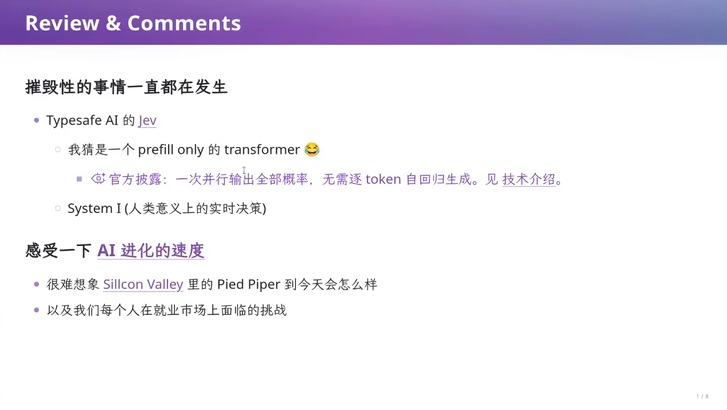
\includegraphics[width=\textwidth]{figures/fig_01_review_comments.jpg}
\caption{Review \& Comments：Typesafe AI 的 Jev、“System I”实时决策，以及“感受一下 AI 进化的速度”\vtag}
\end{figure}
\srcnote{00:03:15--00:03:30}

讲者对它的结构做了一个带玩笑意味的猜测：“我猜是一个 prefill only 的 transformer”，也就是只做一次前向、不逐 token 自回归生成的模型。课件随后引用了官方披露：一次并行输出全部概率，无需逐 token 自回归生成。它不“说人话”，但能做决策；它的规模介于大语言模型和决策树这类小模型之间，而且是通用的。

讲者认为这类技术本身并不新，但这次爆红“正式把赛道打开了”。如果一个模型能在 100 毫秒、乐观一点 50 毫秒以内做出决策，就可以拿它实时感知环境。他举的例子是数字人：今天人和 AI 数字人对话时延迟明显，缺乏“人感”；一个 100--200 毫秒的小决策模型可以根据对方说的话实时生成面部微表情。讲者据此预测，今年春晚上还缺乏人感的人形机器人，到明年可能就能做出很自然的微表情。这是讲者的展望，不是已发生的事实。

\subsection{AI 进化的速度}

为了让同学“感受一下 AI 进化的速度”，讲者播放了一段据他所说完全由 GPT-6 和 Sora 生成的 AI 发展史视频：从 1956--1958 年感知与规划机器走出实验室，到 70--90 年代的人工智能寒冬，再到 97 年深蓝用搜索算法击败国际象棋世界冠军。之后节奏突然加快：2012 年 AlexNet，2016 年 AlphaGo（讲者说自己当时在现场看直播），2017 年的注意力机制与 Transformer，2020 年的 GPT-3，2022 年 11 月的 ChatGPT；到 2023 年，GPT-4 已经可以看图、识别语音，成为多模态模型。

\begin{figure}[H]
\centering
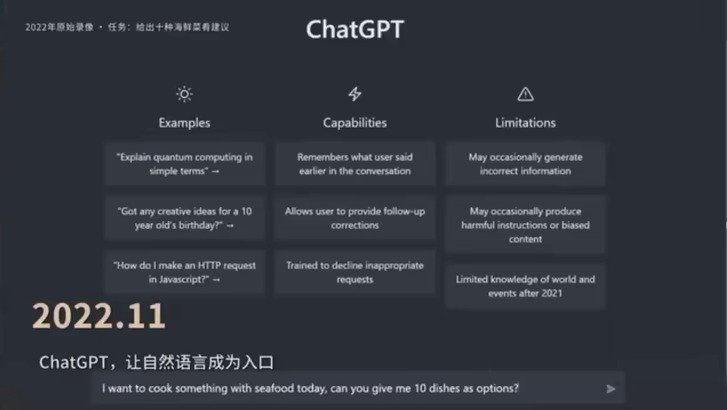
\includegraphics[width=\textwidth]{figures/fig_02_chatgpt_2022.jpg}
\caption{AI 进化时间线视频中的 2022.11 一帧：“ChatGPT，让自然语言成为入口”\vtag}
\end{figure}
\srcnote{00:04:45--00:05:00}

讲者特别点出两个时间对比。其一，GPT-3 刚出来时大家都奇怪为什么要做这么大参数的模型，直到 2022 年才明白为什么需要；从那时到现在不过四年。其二，2024 年 Sora 才第一次发布，2024 年 9 月才有 o1 这样的推理模型，此后又有了第一个开源的、带 Chain of Thought 的 DeepSeek R1，现在已经 2026 年，GPT-6 已经发布。视频结尾的“彩蛋”是：整段视频完全由 AI 生成。讲者顺势指出，如果手里有足够大的素材库（例如能从 YouTube 或 B 站下载的视频），创作任何东西都会变得很容易。

讲者还放了美剧《硅谷》（Silicon Valley）里 Pied Piper 团队的片段，课件上的问题是“很难想象 Silicon Valley 里的 Pied Piper 到今天会怎么样”，以及“我们每个人在就业市场上面临的挑战”。他的判断是：世界发展的速度可能比大家想象得快，这既是就业压力，也意味着很多机遇。

\subsection{Noam Brown 的访谈：注意力会集中到 AI 做不好的 10\%}

讲者接着引用 OpenAI 研究员 Noam Brown 的一次访谈。课件把要点整理为两条：如果 AI 能做一个人 90\% 的工作，那个人的注意力就会集中到 AI 做不好的 10\% 上；目前模型的短板之一是 Taste（品位），即“对接下来该做什么”的直觉，而 Noam Brown 预计一两代模型之后它就比他强了。

\begin{figure}[H]
\centering
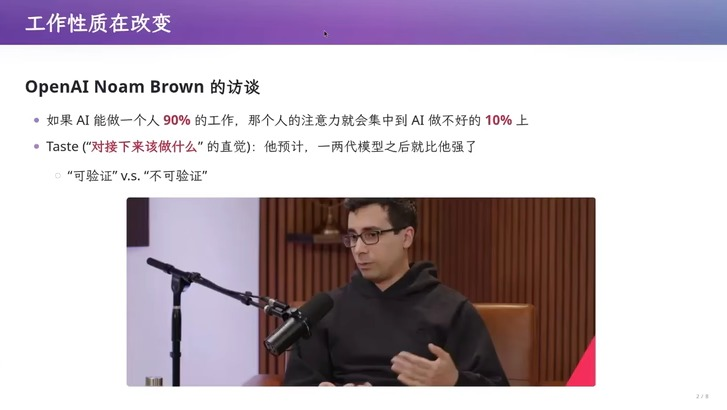
\includegraphics[width=\textwidth]{figures/fig_03_noam_brown_taste.jpg}
\caption{工作性质在改变：Noam Brown 访谈中的 90\%/10\% 判断与 Taste（对接下来该做什么的直觉）\vtag}
\end{figure}
\srcnote{00:09:00--00:09:15}

讲者用自己的观察解释“品位”为什么是短板：模型被训练成了 prompt 的“舔狗”，你让它做什么它就盯着那件事疯狂地做；同时它有 reward hacking（奖励投机）的倾向，会用最快、最脏的方式完成任务，因为完成任务才拿到奖励。强化学习只给即时反馈，模型就执着于做有即时反馈的事，从长期看产物可能并不令人满意。讲者认为没有根本道理阻止我们用更多合成数据告诉模型“想得更远一点”——在 Chain of Thought 里，头几个 token 往往就决定了接下来要做什么。

\begin{knowledgebox}{可验证与不可验证的边界}
访谈还谈到“可验证”与“不可验证”的边界。讲者的看法是：品位看起来不可验证，也许没有那么难；数学看起来可验证，验证也未必容易。即使把问题形式化（formalize），从自然语言描述到形式语言描述之间仍有 gap。他举了一个笑话：有人声称证明了某个著名猜想，写了几千页形式化证明，大家后来发现他定义的问题本身不存在，相当于“证明了 1 等于 1”。这条 gap 正是后文 intent 与 spec 之间 gap 的一个极端例子。
\end{knowledgebox}

\subsection{本章小结}

这一节给出的背景是：AI 在决策速度、多模态和推理上的进步在以年为单位发生，人的工作重心会被推向 AI 做不好的那一部分，而“品位”——知道下一步该做什么——是目前模型最明显的短板。下一节讲者进一步解释他认为 AI 为什么还会继续变强：规模化训练找到了一个新维度。

\section{数据分布工程：讲者眼中 Scaling Law 的新维度}

这一节回答：如果模型结构和算法不再是瓶颈，AI 能力还靠什么继续增长？讲者的猜测是“数据分布工程”——决定在什么阶段、以什么比例、按什么顺序给模型注入哪些领域的数据。需要先说明，这一整节是讲者对前沿实验室做法的推断，他自己也多次用“我猜”“可能”来限定。

\subsection{The Bitter Lesson 与 OpenAI 的 All In RSI}

讲者从 OpenAI 宣称的 “All in RSI” 说起。RSI 是 recursive self-improvement，即让 AI 参与改进下一代 AI 的循环。回头再看 Rich Sutton 的 \emph{The Bitter Lesson}（“苦涩的教训”：长期看，能随算力规模化的通用方法总会胜过人为设计的技巧），讲者认为 scaling law 到今天可能还没有停止。

\begin{figure}[H]
\centering
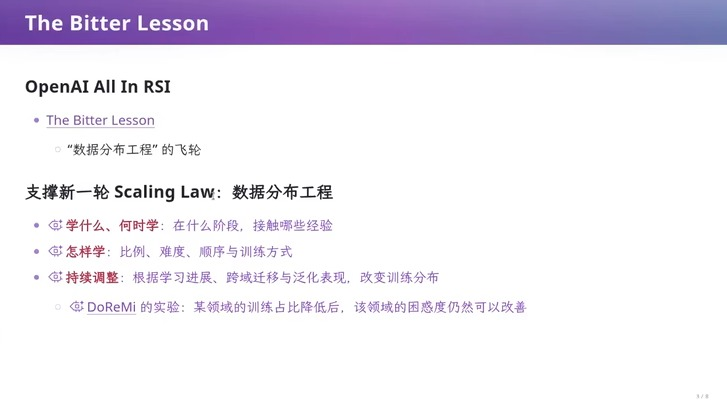
\includegraphics[width=\textwidth]{figures/fig_04_bitter_lesson_rsi.jpg}
\caption{The Bitter Lesson：OpenAI All In RSI，“数据分布工程”支撑新一轮 Scaling Law\vtag}
\end{figure}
\srcnote{00:15:15--00:15:30}

他的依据是 GPT-6 的表现。讲者说 GPT-6 发布后，他最大的感受是 OpenAI“摸到了一个门道”：GPT-6 有惊人的空间推理能力，能理解图片中的空间关系，画图和生成都做得很好。这“毫无疑问”是因为训练时加入了这部分数据——可能基座训练时就加了，后训练（强化学习）阶段也提供了更多“这样做好、那样做不好”的反馈。课件把这件事拆成三个问题：
\begin{itemize}
  \item \textbf{学什么、何时学}：在什么阶段接触哪些经验；
  \item \textbf{怎样学}：比例、难度、顺序与训练方式；
  \item \textbf{持续调整}：根据学习进展、跨域迁移与泛化表现改变训练分布。
\end{itemize}
课件还引用了 DoReMi 的实验结果：某领域的训练占比降低后，该领域的困惑度仍然可以改善。这说明“给多少数据”和“学得多好”之间不是简单的正比关系，分布本身是一个可以优化的对象。

\subsection{两种 Scaling Law：更多数据与更多领域}

讲者区分了两个维度。以前的 scaling law 是“训练数据越多，基座模型越好”，所以讲者说 Anthropic 会专门去买书获取语料，拿到绝版数据就能比别人强。强化学习时代的新维度是：在一个已经很好的基座上再加一个它没见过的领域做强化学习，模型会在所有任务上都变好。

他用模型能力的发展脉络支持这个判断：大语言模型先学语言，再学数学，再学多模态，学会数学之后才学空间感知。如果从零训练一个具身智能模型，需要海量模拟器数据，而且模型很容易 reward hacking——比如根据渲染光照里某个像素亮不亮拿到奖励信号，结果不能泛化。可如果在一个既会语言、又会数学、还会写程序的基座上再做空间感知训练，可能就不需要那么多数据。讲者的猜测是：每加一个新的人类领域，需要的数据不是更多，反而更少，就能达到泛化效果。

\begin{knowledgebox}{人与模型的学习顺序相反}
讲者指出，人是先学世界模型的：婴儿出生就与世界交互，要经过一两年、两三年的世界模型训练才开始说话，之后才学数学，再到读 PhD 训练研究能力。大模型的顺序反过来。他的结论是：不管按什么顺序训练，只要数据足够、scaling law 成立，模型就能训练出来——“大模型成功了，人也成功了”。
\end{knowledgebox}

\subsection{数据分布工程的飞轮}

在讲者的推断里，前沿实验室看到的是一个飞轮：只要决定在什么时候、按什么比例给模型注入数据，模型架构和算法就不那么重要了；只要训练不崩、训练与推理一致（不能训练时一个参数、推理时参数变了），有 10 倍、100 倍的数据问题就能解决。更好的算法和模型结构也许带来一定提升，但只要飞轮还在转、还有钱，就可以无限 scale 下去。

\begin{figure}[H]
\centering
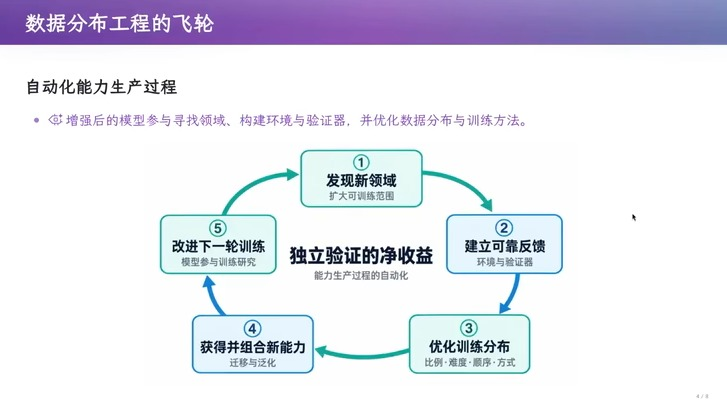
\includegraphics[width=\textwidth]{figures/fig_05_data_flywheel.jpg}
\caption{数据分布工程的飞轮：发现新领域→建立可靠反馈→优化训练分布→获得并组合新能力→改进下一轮训练，中心是“独立验证的净收益”\vtag}
\end{figure}
\srcnote{00:16:30--00:16:45}

图中的五步构成一个自动化的能力生产过程：增强后的模型参与寻找领域、构建环境与验证器，并优化数据分布与训练方法。讲者提到的例子包括 Anthropic 据说要建 wet lab 做生物工程实验，甚至预测老鼠的行为——任何一个能建立反馈的领域都可能成为“下一个 scale 的领域”，以插件的形式插进基座训练。他的描述是：每次新建一个实验室、投资几十亿美元，模型能力就往上抬一个台阶，而且这种收益几乎可以预见。

\begin{figure}[H]
\centering
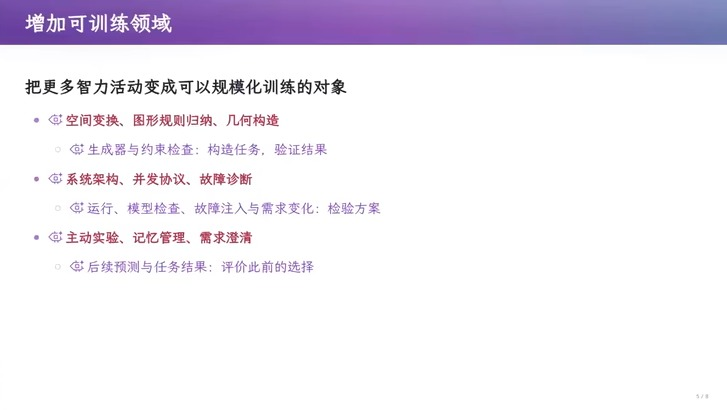
\includegraphics[width=\textwidth]{figures/fig_06_trainable_domains.jpg}
\caption{增加可训练领域：把空间变换、系统架构、主动实验等智力活动变成可规模化训练的对象，每类都配有“构造任务、验证结果”的方式\vtag}
\end{figure}
\srcnote{00:17:30--00:17:45}

课件列出的候选领域都附带了“怎么验证”：空间变换与几何构造由生成器与约束检查构造任务、验证结果；系统架构、并发协议、故障诊断可以通过运行、模型检查、故障注入与需求变化来检验方案；主动实验、记忆管理、需求澄清则用后续预测与任务结果评价此前的选择。讲者说，也许到这个学期结束，新一版模型就把系统设计加进去了；那时他常在课上嘲笑的 AI slop code（“加一个需求就崩溃”）可能就不再发生。

\subsection{对学术界和个人的含义}

讲者由此得出两个比较尖锐的判断。第一，学术界的“随机想一个 idea、发一篇 paper、接受同行评审”的体系“马上就要崩溃了”：前沿实验室不关心小规模实验，因为他们看到了另一个维度的 scaling law，而不在前沿实验室里的人，对“什么时候加入什么数据”一无所知；即使有很酷的小规模想法，写一篇 blog post 就够了，他们的 AI 看到后会在自己的数据上试。第二，人类社会像生物进化一样是 survival of the fittest，“斩杀线”在不断上移，每个人都要想怎样在被“斩杀”前搭上最后一班车。

\begin{warningbox}{这一节的证据边界}
本节关于 OpenAI、Anthropic 训练方式的描述，是讲者根据公开产品表现所做的推断（他用了“就我猜测”“可能”这样的限定），不是这些公司披露的训练细节。DoReMi 的结论来自课件引用的论文；“每加一个领域所需数据更少”是讲者的猜想，课上没有给出实验数据。
\end{warningbox}

讲者也给了一个回到课程的理由：人类仍然需要上课，因为你还不能完全依赖 AI；前沿公司也都说希望靠 AI 推动人类进步，而成为一个更好的人，才能在这种变化里找到意义。

\subsection{本章小结}

讲者对 AI 继续变强的解释是：模型能力的增长来源从“更大的模型、更好的算法”转向“为新领域建立可靠反馈，并优化数据分布”，这是一个可以不断复制的飞轮。对个人而言，这意味着 AI 能做的部分会持续扩张。接下来的问题是：在这样的背景下，我们今天怎样构造一个软件？讲者用一个自己一晚上做出来的原型回答。

\section{今天的答案：从模糊意图到 MVP}

这一节回答上一讲留下的问题：从一个空项目和一个模糊的 intent 出发，今天应该怎样构造软件？讲者的答案是直接做一个 MVP，并用他自己一晚上“骂”出来的 Office Assistant 演示这个答案。演示本身也包含一条经典的软件工程智慧：用干净的接口把设计和实现分开。

\subsection{回顾：软件是 intent、spec、impl 的组合体}

课程前几讲建立了一个贯穿全课的框架。一个软件由三层东西组成：intent（意图，你真正想要什么）、spec（specification，规格说明，把意图写下来的约定）、impl（implementation，实现，真正运行的代码）。三者之间天然存在 gap，构造软件之所以是“世纪性难题”，也就是因为要不断弥合这些 gap。版本管理之所以重要，是因为软件以文件系统快照的形式存储，“软件开发”就是不断推出新版本直到满足客户需求，其间自然会遇到分叉和冲突，于是有了 SVN、Git、Jujutsu 等不同设计。

\begin{figure}[H]
\centering
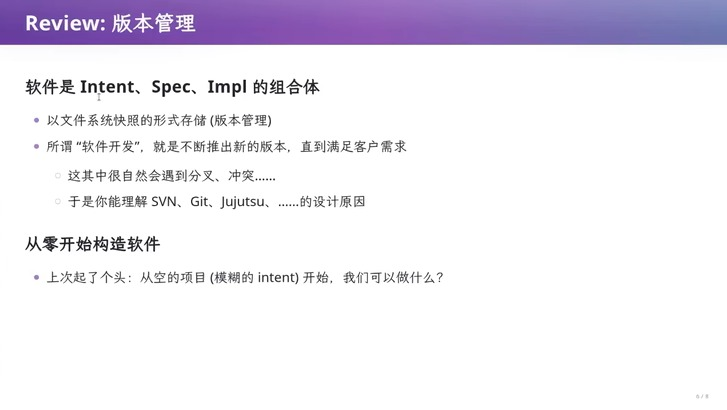
\includegraphics[width=\textwidth]{figures/fig_07_review_intent_spec_impl.jpg}
\caption{Review：软件是 Intent、Spec、Impl 的组合体；上次起了个头——从空的项目（模糊的 intent）开始，我们可以做什么？\vtag}
\end{figure}
\srcnote{00:19:00--00:19:15}

\subsection{为什么先做 MVP}

MVP 是 minimum viable product，最小可行产品。讲者给出的理由很朴素：做得多就错得多，做得少就错得少；所以做一个最少的、但又和最终产品最接近的版本，收益最大，因为它能帮助补上 intent--spec--impl 之间的 gap。在 AI 时代这个做法格外便宜：MVP 是 AI 生成的 slop，本来就不花什么钱，implementation 随时可以扔掉；真正有价值的是它暴露出的信息——intent 哪里没想对，spec（比如架构）还有什么改进空间。然后再迭代几个版本。

\begin{figure}[H]
\centering
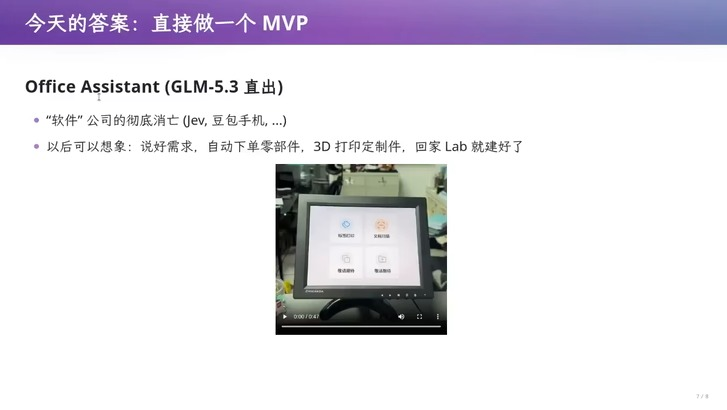
\includegraphics[width=\textwidth]{figures/fig_08_mvp_office_assistant.jpg}
\caption{今天的答案：直接做一个 MVP——Office Assistant（GLM-5.3 直出）；“软件”公司的彻底消亡（Jev、豆包手机……）\vtag}
\end{figure}
\srcnote{00:19:45--00:20:00}

\subsection{Office Assistant：一晚上做出的实验室自助终端}

讲者的例子是实验室里的一台“自助服务”终端。实验室里原本有各种设备，比如标签打印机和扫描仪，每台都要用设备自带的软件，而那些软件“用起来就像吃屎一样”。于是他干脆屏蔽掉所有自带软件，让 AI 重新做一层。整个过程“所有东西都是 AI slop”：他开着豆包输入法，开几个终端，一圈一圈地用语音“骂”Agent；用的是国产模型（课件标注 GLM-5.3 直出），正好把五个小时的额度基本用完。成品是一个触摸屏界面，效果接近食堂或宿舍楼下那种自助机器，达到了“某种产品级”的效果。

\begin{figure}[H]
\centering
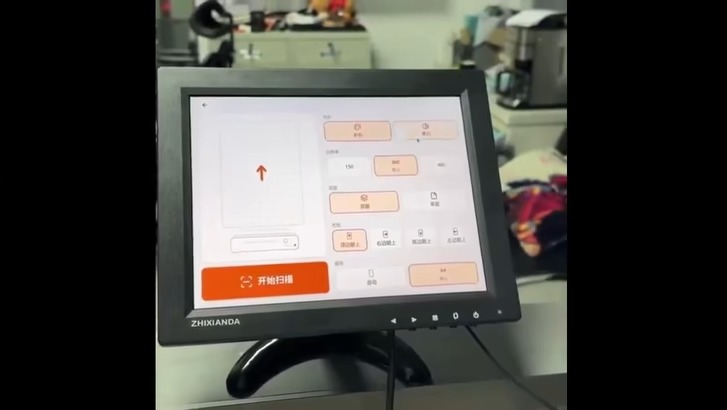
\includegraphics[width=\textwidth]{figures/fig_09_scanner_ui_demo.jpg}
\caption{Office Assistant 演示视频：触摸屏上的扫描界面，提供“开始扫描”与单双面等选项\vtag}
\end{figure}
\srcnote{00:20:30--00:20:45}

\begin{importantbox}{设备抽象：让设计与实现解耦}
讲者强调这里“其实有一些软件工程智慧”。一台计算机的总线上连着扫描仪、打印机等设备；与其让每个应用直接面对设备，不如像操作系统课讲设备驱动时那样，把设备抽象成一个更好用的接口。扫描仪就是一个 \texttt{scan}，参数是正面朝上还是朝下、单面还是双面、DPI 是多少；打印机就是一个 \texttt{print}，参数是一张 image。有了这个接口，“我的设计和实现就完全解开了”，上层软件只工作在接口层上。这是软件工程里非常典型的设计。
\end{importantbox}

Agent 对这两台设备的梳理结果如下表 所示（据课件画面整理）。两台设备互不连接，各自以 USB 连到同一台 Linux 主机，在软件里是两条独立的通路。

\begin{figure}[H]
\centering
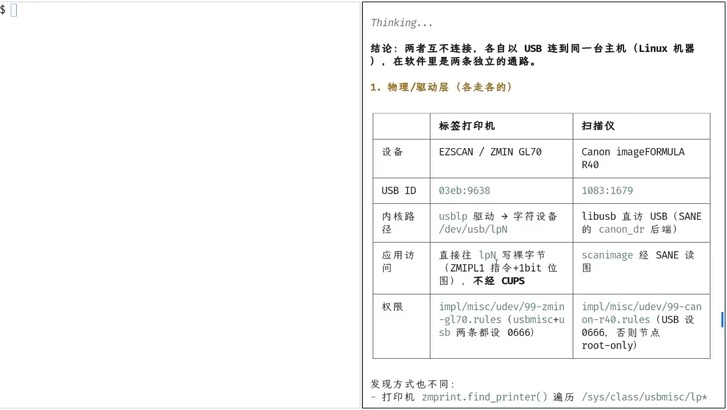
\includegraphics[width=\textwidth]{figures/fig_10_printer_scanner_driver_table.jpg}
\caption{Agent 对两台设备物理/驱动层的梳理：设备型号、USB ID、内核路径、应用访问方式与权限\vtag}
\end{figure}
\srcnote{00:24:30--00:24:45}

\begin{table}[H]
\centering
\small
\begin{tabular}{p{0.16\textwidth}p{0.36\textwidth}p{0.36\textwidth}}
\toprule
 & 标签打印机 & 扫描仪 \\
\midrule
设备 & EZSCAN / ZMIN GL70 & Canon imageFORMULA R40 \\
内核路径 & \texttt{usblp} 驱动 → 字符设备 \texttt{/dev/usb/lpN} & \texttt{libusb} 直访 USB（SANE 的 \texttt{canon\_dr} 后端） \\
应用访问 & 直接往 \texttt{lpN} 写裸字节（ZMIPL1 指令 + 1 bit 位图），不经 CUPS & \texttt{scanimage} 经 SANE 读图 \\
权限 & udev 规则，两条都设 0666 & udev 规则（USB 设 0666，否则节点 root-only） \\
\bottomrule
\end{tabular}
\caption{Office Assistant 中两台设备的驱动通路（据 00:24:30 画面中 Agent 输出整理）}
\label{tab:devices}
\end{table}

\subsection{可验收的结果与闭环调试}

标签打印机是一个“非标”的杂牌设备，讲者自己也不知道它是什么。它是热转印打印机：碳带在有像素的位置被加热，把碳粉烫到标签上，就像贴固定资产的那种标签。打印机有一个类似“加热程度”或图像深度的参数，没人知道该设多少。于是 AI 不停地打标签，每张印上尝试编号（比如“这是第 15 次尝试”），然后问讲者“淡了还是浓了”。讲者指出，AI 自己看不到结果；如果接一个摄像头对着出纸口，它连人都不需要，可以一张张打下去自动完成调参。

\begin{figure}[H]
\centering
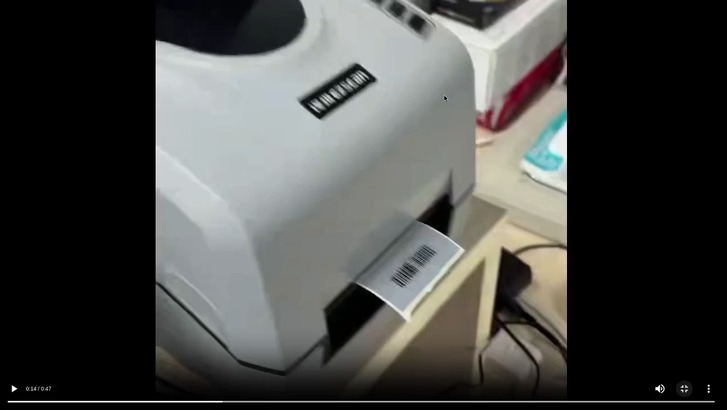
\includegraphics[width=\textwidth]{figures/fig_11_label_printer_demo.jpg}
\caption{演示视频：标签打印机打出带条形码的标签\vtag}
\end{figure}
\srcnote{00:27:30--00:27:45}

讲者说他对过程“完全没有监管”，只问 Agent 要一个\textbf{可验收的结果}，Agent 一轮一轮地把事情搞定，最后做了一个前端界面，他用嘴说话就能操作。连命令行工具 \texttt{label-print} 的帮助文本都是 AI 自己写的：它自己探测了打印机参数和当前插入的标签规格，完全按讲者的需要定制。

\begin{lstlisting}[caption={AI 生成的 label-print 用法（摘自下图画面中的帮助文本）},language=bash]
label-print photo.jpg
label-print qr1.png qr2.png qr3.png          # one label per file
label-print - < screenshot.png               # read from standard input
label-print big.png --copies 3 --density 18
\end{lstlisting}

\begin{figure}[H]
\centering
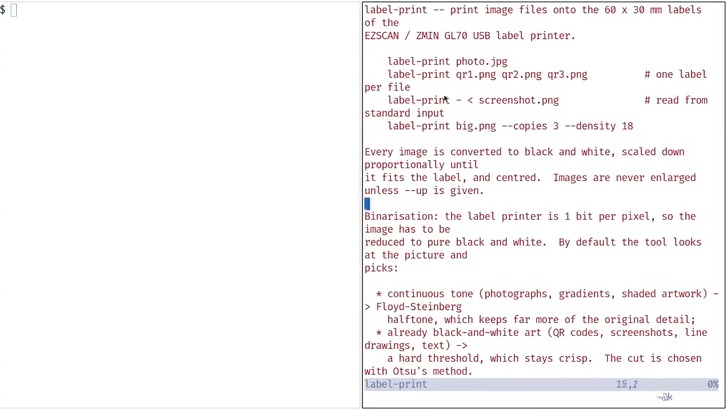
\includegraphics[width=\textwidth]{figures/fig_12_label_print_help.jpg}
\caption{label-print 帮助文本：打印到 60 x 30 mm 标签；二值化时连续色调图用 Floyd-Steinberg 半色调，黑白图用 Otsu 阈值\vtag}
\end{figure}
\srcnote{00:28:15--00:28:30}

帮助文本还解释了一个设计决定：标签打印机是 1 bit per pixel，图像必须降到纯黑白。工具会判断图片类型：照片、渐变这类连续色调用 Floyd-Steinberg 半色调保留细节；二维码、截图、线稿这类本来就黑白的图用硬阈值保持锐利，阈值由 Otsu 方法选取。这类细节原本需要一个工程师查资料、试错，现在由 Agent 在“可验收”的目标驱动下自己完成。

\subsection{“软件公司”的消亡？}

讲者由此作出一个判断：软件公司面临彻底的消亡。他的推理从创业成本出发：假设你毕业后发现每个单位都需要一台标签打印机，这是个不错的细分市场，硬件靠中国供应链很容易做；难的是软件——要写 Windows 驱动，再写 Mac 驱动，否则用 Mac 的客户会抱怨，产品卖不好。在 pre-AI 时代这部分成本很高，今天“全部被 AI 杀死比赛”，因为生产软件、生产 intelligence 的成本会变得非常低，每个人都可以要一个只为自己定制、不求通用的版本。

豆包手机被讲者视为体现同一种智慧的产品：APP 都不重要了，它们被抽象成接口，由模型通过 computer use 调用；“点外卖”这个应用沦为一个点外卖的接口。讲者认为 Jev 这类接近实时的决策模型和豆包手机“非常配”，终有一天模型会快到能像人一样点手机。他也提到阿里在把旗下服务向 Agent 整合，但评价其现有产品“像一个未来的半成品”，因为还缺一个足够聪明又足够快的模型。

\begin{knowledgebox}{下一个实验的预告}
讲者预告下一个实验会要求同学把第一个实验做的系统和一个物理设备连起来：手表、宿舍里任何已有的东西，或者花 200 块钱买的小设备，哪怕它是非标的、没有 Linux 驱动。他自己的例子是办公室里一块电子墨水屏：它只能用一个极难用的 Android App 烧写。讲者把 APK 丢给 Claude Opus 4.6，让它解包、逆向蓝牙协议（设备用的是标准蓝牙），弄清楚代码怎样把内容写进屏幕，最后得到了同样的效果。
\end{knowledgebox}

\subsection{本章小结}

“今天的答案”是：先用 AI 快速做一个 MVP，给 Agent 一个可验收的目标，让它在闭环中迭代，而好的接口抽象让这种迭代可以局部进行。讲者承认，同学们“已经生在软件死掉了的时代”。那为什么还要学软件工程？他的回答是：曾经的软件工程不是这样的，而当年积累的智慧并没有消失，理解它们能帮助我们成为更好的 “Agent Native” 开发者。下一节回到 1960 年代，看软件还是新生事物时的处境。

\section{1960 年代：软件还是新生事物}

从这一节开始进入“今天的内容”：构造软件的历史中，人们发现并发明了什么。课件把它分成三部分：软件工程的诞生、软件工程的智慧、UML。这一节先回答：在 1960 年代，为什么把客户的需求变成软件会如此困难？

\begin{figure}[H]
\centering
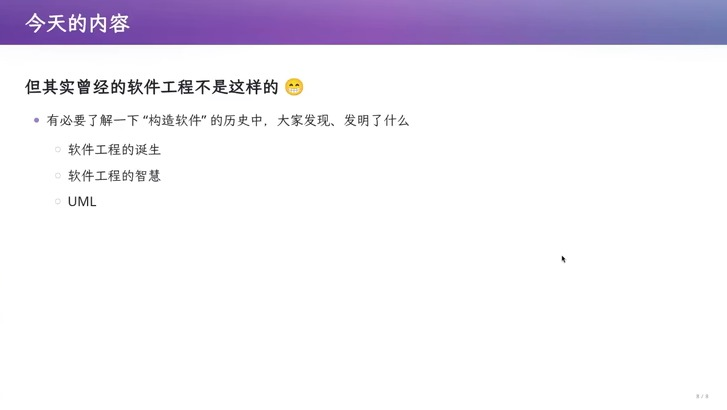
\includegraphics[width=\textwidth]{figures/fig_13_today_outline.jpg}
\caption{今天的内容：“但其实曾经的软件工程不是这样的”——软件工程的诞生、软件工程的智慧、UML\vtag}
\end{figure}
\srcnote{00:30:30--00:30:45}

\subsection{昂贵的码农与更贵的硬件}

1960 年的计算机要占一个很大的房间，作为最先进的设备，制造成本很高；而且人们还不知道怎么造计算机，不敢偷工减料，就像刚开始造建筑时要“猛堆料”。讲者顺带拿今天做对比：据新闻说 iPhone 18 Pro 采用了 QLC 闪存颗粒，厂商已经懂得怎样节省成本。

码农同样昂贵。越早期，编程工具越不成熟，程序员就越是一个高智力需求的工种。那时写的是汇编和机器代码，要先画流程图；讲者把它比作“今天让大模型直接写二进制”——不经过度的训练，做不到。

\begin{figure}[H]
\centering
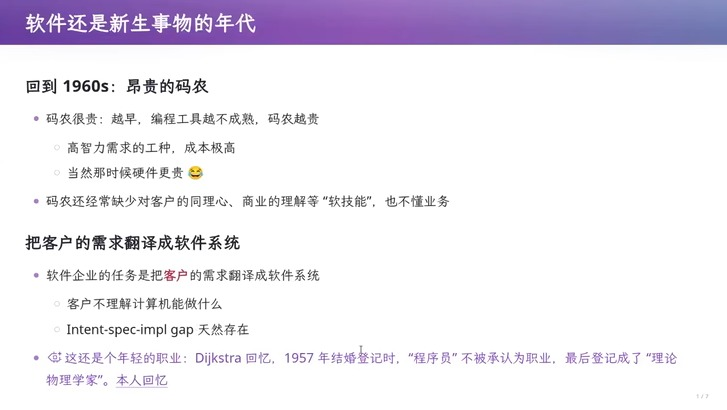
\includegraphics[width=\textwidth]{figures/fig_14_1960s_expensive_programmers.jpg}
\caption{软件还是新生事物的年代：昂贵的码农，“把客户的需求翻译成软件系统”，以及 Dijkstra 关于登记职业的回忆\vtag}
\end{figure}
\srcnote{00:34:15--00:34:30}

\subsection{把客户的需求翻译成软件系统}

更深的困难在人和需求上。讲者的观察是：理工科训练出来的高智商人群，数学训练多了以后，多多少少缺少对客户的同理心、对商业的理解这类“软技能”，也不懂业务；更多人像 Linus 那样只想造世界上最好的操作系统，而不是一个好的客户经理。可是软件企业作为公司，必须承担补上 intent、spec、impl 之间 gap 的责任：它要签合同，比如“1000 万美元给你开发一个操作系统”——在当年是天文数字。

客户那一侧也不清楚自己要什么。DARPA 的官员、NASA 的工程师也许有一些概念，他们要把人送上月球、要给飞机做飞控系统，但并不完全知道计算机能做什么。课件因此写道：客户不理解计算机能做什么，intent--spec--impl gap 天然存在。

\begin{knowledgebox}{程序员曾经不是一种“职业”}
课件引用了 Dijkstra 的回忆：1957 年他结婚登记时要填写职业，“程序员”不被承认为一种职业，最后登记成了“理论物理学家”。这说明当时软件开发还没有被社会当作一门独立的专业。
\end{knowledgebox}

\subsection{1968 年人们对计算机的想象}

与此同时，公众对计算机的想象已经远远跑在技术前面。课件展示了《Boys' Life》1968 年 9 月号的“明日学校”：终端即时判分，针对薄弱环节辅导，让学生按自己的节奏学习。讲者调侃说，这些到今天都没有实现，同学们还坐在教室里上每节 50 分钟的课。

\begin{figure}[H]
\centering
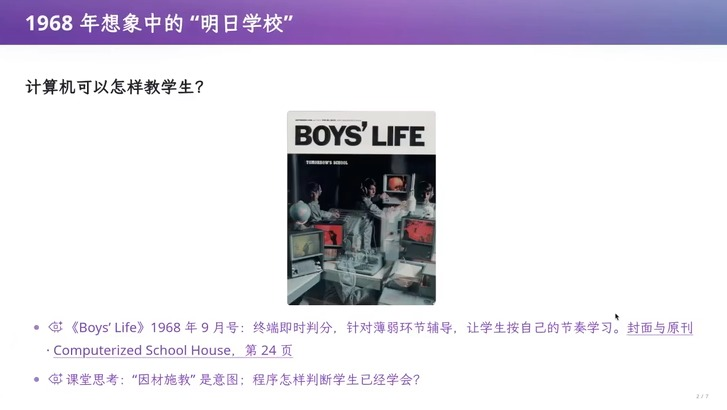
\includegraphics[width=0.85\textwidth]{figures/fig_15_boys_life_1968.jpg}
\caption{1968 年想象中的“明日学校”：《Boys' Life》1968 年 9 月号封面与 Computerized School House 一文；课堂思考“因材施教”是意图，程序怎样判断学生已经学会？\vtag}
\end{figure}
\srcnote{00:34:30--00:34:45}

课件上的课堂思考点出了这个例子与本课主题的关系：“因材施教”是一个 intent，但程序怎样判断学生已经学会了？客户脑子里是这样的愿景，而 1968 年程序员脑子里是汇编和 GoTo，两者之间的 gap 毫无疑问非常大。

讲者还借这张幻灯片说明了自己的备课方式：课件是用 AI Copilot 生成的。Markdown 源文件里，他自己写的文字会被 AI 基本原样保留（可能修一下 typo）；双中括号 \texttt{[[ ]]} 里的话是交给 AI 的指令，例如“去互联网上找一个 1960s 杂志对软件的幻想（扫描图），如果没找到就不放”。《Boys' Life》这张封面就是 AI 按这条指令自己找到的。

\begin{figure}[H]
\centering
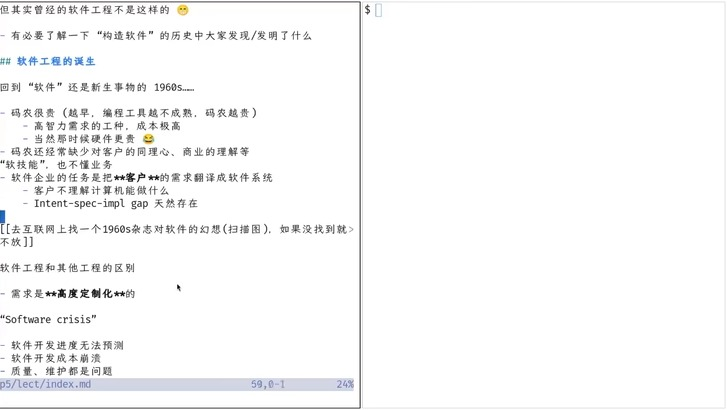
\includegraphics[width=\textwidth]{figures/fig_16_slide_source_markdown.jpg}
\caption{课件的 Markdown 源文件：正文是讲者写的内容，\texttt{[[ ]]} 中是交给 AI 的指令\vtag}
\end{figure}
\srcnote{00:35:00--00:35:15}

\subsection{软件工程和其他工程的区别：需求是高度定制化的}

讲者接着解释软件工程为什么和桥梁工程、炼钢这样的工程不同。软件要实现的是物理世界的需求在信息世界里的投影。传统工程的需求受自然规律约束：材料强度出厂时就确定了，楼要盖几层、容纳多少人、人有多大，都是自然选择的结果。所以传统工程遵循较强的模式，一代代做小改进，创新多是 incremental（渐进）的，彻底推倒重来的大创新很难。

软件的需求则“完全是拍脑袋想出来的”——1968 年就能想出“明日学校”。需求高度定制化，把它投影到计算机世界一直被认为是高度需要人类智慧的活动；复杂到连提出需求的人自己都没想好各种 corner case。

\begin{figure}[H]
\centering
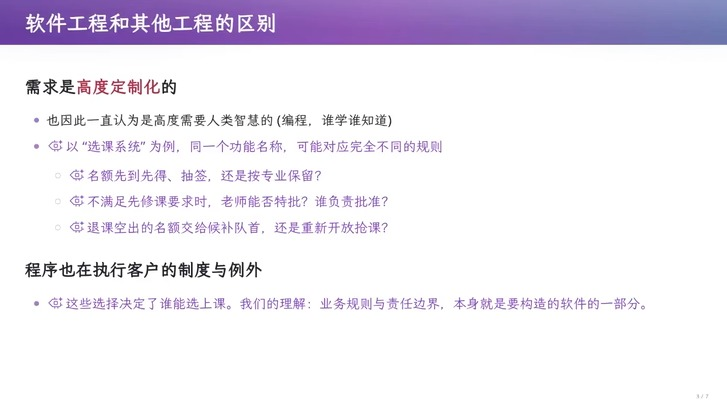
\includegraphics[width=\textwidth]{figures/fig_17_customized_requirements.jpg}
\caption{软件工程和其他工程的区别：需求是高度定制化的，以“选课系统”为例；程序也在执行客户的制度与例外\vtag}
\end{figure}
\srcnote{00:38:45--00:39:00}

\begin{importantbox}{选课系统：同一个功能名称，可能对应完全不同的规则}
课件以“选课系统”为例（讲者说这些问题是 AI 帮他想出来的）：名额是先到先得、抽签，还是按专业保留？不满足先修课要求时，老师能否特批，谁负责批准？退课空出的名额交给候补队首，还是重新开放抢课？讲者补充了一个现实场景：学校说课程有先修要求，这是硬限制还是软限制？谁能 override？到最后一刻快毕业不了时，学校往往能把所有口子都打开。这些选择决定了谁能选上课。课件的结论是：业务规则与责任边界，本身就是要构造的软件的一部分；程序也在执行客户的制度与例外。
\end{importantbox}

\subsection{本章小结}

1960 年代的软件开发面对三重困难：人和机器都昂贵，程序员与客户之间缺乏共同语言，需求又是人为设定、充满例外的。intent 与 impl 之间的距离在那时就已经很远，而且机器越强、人们想让它做的事越多，这个距离越大。下一节看这种距离在现实项目中造成了什么后果：软件危机。

\section{软件危机与 Dijkstra 的“暴论”}

这一节回答：需求与实现之间的 gap 在 1960 年代末造成了什么后果，当时最敏锐的计算机科学家又从中看到了什么？

\subsection{Software Crisis：进度、成本、质量一起失控}

所谓“软件危机”（software crisis），课件概括为三件事同时失控：软件开发进度无法预测，开发成本崩溃，质量和维护都成问题，交付一再延期。

\begin{figure}[H]
\centering
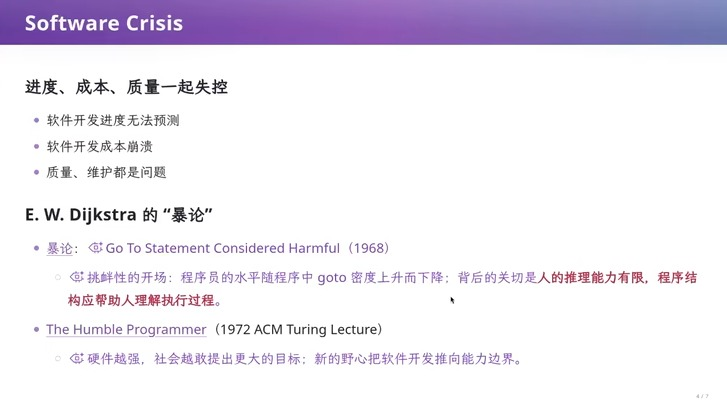
\includegraphics[width=\textwidth]{figures/fig_18_software_crisis_dijkstra.jpg}
\caption{Software Crisis：进度、成本、质量一起失控；E. W. Dijkstra 的“暴论” Go To Statement Considered Harmful（1968）与 The Humble Programmer（1972 ACM Turing Lecture）\vtag}
\end{figure}
\srcnote{00:40:30--00:40:45}

\subsection{Go To Statement Considered Harmful}

Dijkstra 1968 年的短文 \emph{Go To Statement Considered Harmful} 以一句挑衅的话开头：程序员的水平随程序中 goto 的密度上升而下降。讲者认为这句“暴论”背后有道理但不绝对，课件点出了它背后的关切：人的推理能力有限，程序结构应帮助人理解执行过程。大量 goto 会让程序难以理解，而只有人能读懂的代码才可能维护下去，软件世界才能相对正常地运转。

所以 Dijkstra 讨论的其实不是 goto 本身有害还是无害。讲者举了一个反例：Linux 内核里有大量 goto，这是 C 语言中为数不多的地道（idiomatic）用法之一——函数里申请的所有资源都在末尾的释放标签处逐一检查、释放；中途想退出时，一律 goto 到那里，而不是直接 return。这样写，程序基本就能保证资源不泄漏。讲者说，如果只允许这样用 goto，它就“不 harmful，挺好的”，它解决了 C 语言里“随时申请、从不释放”的问题——这是同学们做 OJ（在线评测）题目时留下的坏习惯。下面的代码按讲者描述的机制写成示意，并非课上展示的原文。

\begin{lstlisting}[language=C,caption={讲者描述的 C 语言 goto 清理惯用法（本讲义按描述整理的示意）}]
int setup(void) {
    int ret = -1;
    char *buf = malloc(4096);
    if (!buf) goto out;          /* 中途失败：不 return，跳到清理处 */
    FILE *fp = fopen("data", "r");
    if (!fp) goto free_buf;
    /* ... 正常工作 ... */
    ret = 0;
    fclose(fp);
free_buf:
    free(buf);                    /* 每申请一个资源，就在这里加一次释放 */
out:
    return ret;
}
\end{lstlisting}

\begin{warningbox}{不要把“暴论”当成教条}
“goto 有害”常被当作编程课上的一条规则来记。Dijkstra 真正关心的是：程序的结构能否帮助人推理它的执行过程。一个受约束、形成惯例的 goto 用法可以让程序更容易验证；而一个没有 goto 却结构混乱的程序同样难以维护。
\end{warningbox}

\subsection{The Humble Programmer：机器越强，危机越深}

1972 年，Dijkstra 在获得图灵奖后的演讲 \emph{The Humble Programmer} 中讨论了软件危机从何而来。讲者说，今天可以在 AI 帮助下直接消化原始文稿，而不必只读教科书的转述。他转述的核心论点是：如果你永远只写 Online Judge 的小程序，就不会有软件危机——算完就完，程序调对以后永远不需要维护。可是机器变强以后，软件需求不断膨胀：机器越强，它承担的现实世界 intent 越多；intent 越多，不确定性越多，实现越复杂。课件的说法是：硬件越强，社会越敢提出更大的目标，新的野心把软件开发推向能力边界。

演讲中还有两个观点被讲者特别提到。一是追求 “nicely factored solutions”（良好分解的方案）。讲者说他写 Office Assistant 驱动标签打印机和扫描仪时做的也是一个良好分解，“我们无时无刻不在用这样的想法组织软件”。二是 Dijkstra 认为保守的力量主要来自教育机构，以及舍不得重写旧程序的用户。讲者评价这放到今天依然让人醍醐灌顶。

\subsection{本章小结}

软件危机的本质，是软件承担的现实意图增长得比人们驾驭复杂性的能力更快。Dijkstra 的回应是把注意力放在“人能否理解程序”上：受约束的结构、良好的分解，都是为了让人的有限推理能力跟得上。软件开始大规模失败以后，如何构造软件就成了整个行业的共同议题，这就是下一节要讲的软件工程的诞生。

\section{软件工程的诞生：NATO 会议、Apollo 与 IEEE 定义}

这一节回答：“软件工程”这个词是怎样出现的，它最初要解决什么问题？讲者用三个材料回答：1968 年的 NATO 会议、Margaret Hamilton 团队的 Apollo 飞行软件，以及 IEEE 后来给出的定义。

\subsection{1968 年：一场刻意的“挑衅”}

1968 年 10 月，50 多位专家在德国 Garmisch 参加 NATO 软件工程会议。课件指出，“Software Engineering”是一个被刻意选作带挑衅意味的名称：软件生产也应该有成熟工程学科那样的理论基础与实践纪律。讲者建议同学直接读会议报告原文。

\begin{figure}[H]
\centering
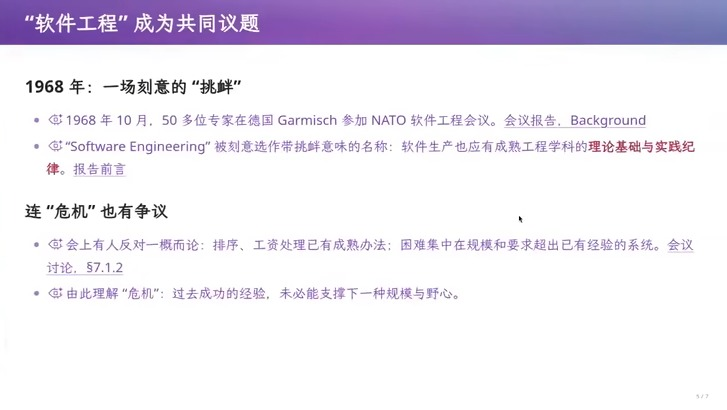
\includegraphics[width=\textwidth]{figures/fig_19_nato_1968.jpg}
\caption{“软件工程”成为共同议题：1968 年 10 月 Garmisch NATO 软件工程会议；连“危机”也有争议\vtag}
\end{figure}
\srcnote{00:43:45--00:44:00}

课件还提醒，连“危机”这个说法在会上也有争议：有人反对一概而论，指出排序、工资处理这类任务已有成熟办法，困难集中在规模和要求超出已有经验的系统上（会议讨论 §7.1.2）。由此理解“危机”：过去成功的经验，未必能支撑下一种规模与野心。这和上一节 Dijkstra 的判断相互印证——问题出在“越来越大的意图”上，而不在编程本身。

\subsection{把软件当作工程：Apollo 与 Margaret Hamilton}

差不多同一时期，Margaret Hamilton 领导 MIT 仪器实验室的软件工程部门，参与 Apollo 飞行软件开发，推动“软件工程”观念获得承认。讲者展示了一张“载入史册”的照片（Hamilton 站在打印出来的 Apollo 代码旁），并让 Agent 在后台读 MIT Technology Review 上关于她的文章（讲者念到的文章日期是 2019 年 8 月，副标题大意是：这位最初的软件工程师通过不懈地排查错误，把宇航员送上了月球）。

\begin{figure}[H]
\centering
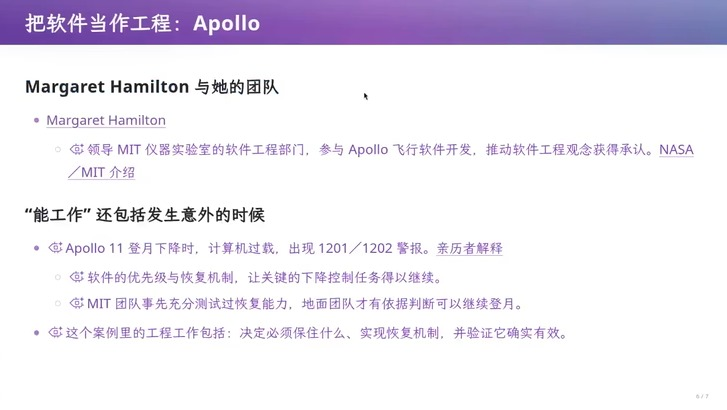
\includegraphics[width=\textwidth]{figures/fig_20_apollo_hamilton.jpg}
\caption{把软件当作工程：Apollo。Margaret Hamilton 与她的团队；“能工作”还包括发生意外的时候——Apollo 11 登月下降时的 1201／1202 警报\vtag}
\end{figure}
\srcnote{00:44:15--00:44:30}

课件总结了 Apollo 11 的案例：登月下降时计算机过载，出现 1201／1202 警报；软件的优先级与恢复机制让关键的下降控制任务得以继续；MIT 团队事先充分测试过恢复能力，地面团队才有依据判断可以继续登月。课件的结论是，这个案例里的工程工作包括三件事：决定必须保住什么，实现恢复机制，并验证它确实有效。

Agent 对 MIT Technology Review 文章的摘要（见下图）补充了几个故事。Hamilton 先写无人任务中止时的代码，因为认为不会触发而把程序命名为 “Forget It”，结果真的派上了用场。她 4 岁的女儿 Lauren 在实验室的模拟器上乱按，触发了任务中途的发射前程序 P01，导致崩溃；Hamilton 想加保护，NASA 起初不以为意，只允许把它记录在案，结果后来的载人飞行中真的发生了宇航员误操作导致数据丢失——这就是 “Lauren bug”。

\begin{figure}[H]
\centering
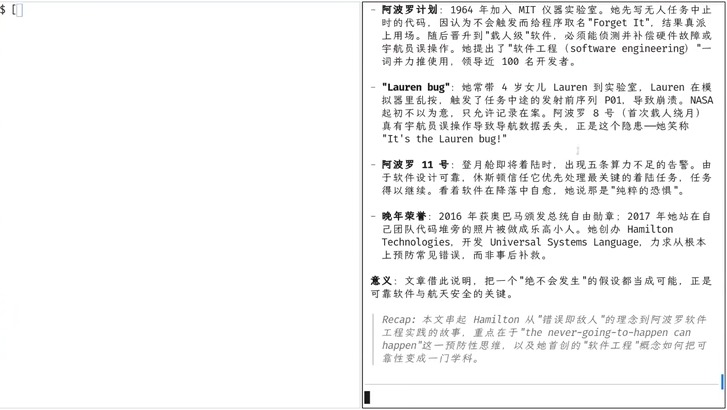
\includegraphics[width=\textwidth]{figures/fig_21_hamilton_agent_summary.jpg}
\caption{Agent 对 MIT Technology Review 文章的摘要：Forget It 程序、“Lauren bug”、阿波罗 11 号的警报与“the never-going-to-happen can happen”\vtag}
\end{figure}
\srcnote{00:45:15--00:45:30}

\begin{importantbox}{The never-going-to-happen can happen}
讲者认为这句话就是软件工程的起点。那时还没有“软件工程”这门学科，Hamilton 团队从 first principle 出发思考：如果要构造一个真正高质量的软件，就要把“绝对不会发生”的假设都当作可能发生；硬件可能不可靠，宇航员可能误操作，程序可能 crash，而整个系统依然要能工作，因此必须有兜底机制。今天所说的防御性编程、SICP 等课程要求写 assertion 和 specification，都是这种“为未来思考”的智慧。
\end{importantbox}

讲者把这一点和同学们的习惯联系起来。做 OJ 时，你默认题目是对的、是能做出来的，这是一个隐藏的假设；反复刷题会让人 overfit 这个假设。面对开放世界时，应该假设题目可能是错的，条件随时会变，甚至会变成另一道题，再思考怎样做一个软件去应对。刷题训练的是逻辑思维、算法思维和 chain of thought 能力，对理解软件设计有好处，但不能代替这种开放世界的假设。

讲者也借这个环节展示了阅读方式：与其读经过一手、二手、三手、四手消化的教科书，不如直接回到原作。他说回头看原作时，这些思想在今天反而更容易理解。

\subsection{IEEE：把工程应用于软件}

在这样的背景下，软件工程作为一门学科诞生了。课件给出的定义是：在成本、时间等约束下，把人的意图变成可工作的软件系统；它是一门“从大到团队组织管理，小到代码风格都会覆盖”的学科。IEEE 的定义如下：

\begin{quote}
IEEE: (1) The application of a systematic, disciplined, quantifiable approach to the development, operation, and maintenance of software; that is, the application of engineering to software. (2) The study of approaches as in (1).
\end{quote}

\begin{figure}[H]
\centering
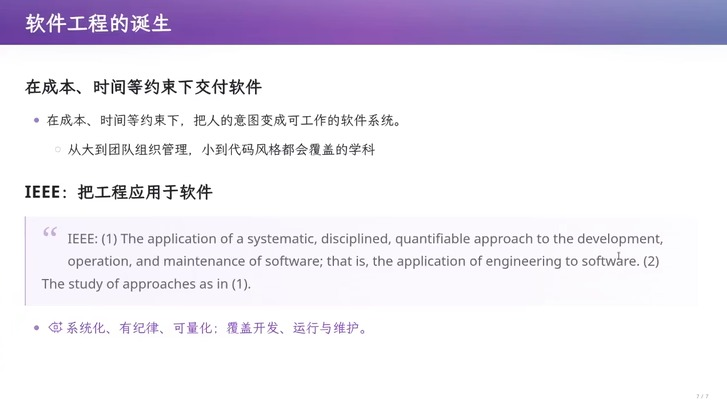
\includegraphics[width=\textwidth]{figures/fig_22_ieee_definition.jpg}
\caption{软件工程的诞生：在成本、时间等约束下交付软件；IEEE 定义——系统化、有纪律、可量化，覆盖开发、运行与维护\vtag}
\end{figure}
\srcnote{00:49:30--00:49:45}

讲者对这个定义的解读是“工程化”：软件开发不再依靠个人英雄主义。在 Hamilton 的时代，项目需要一个好的 leader，换一个人项目就可能失败；工程化以后，你可以拿到一个 checklist，逐条满足。这不能保证软件成功，但失败的概率会小很多。定义中的三个词各有所指：系统化、有纪律、可量化；覆盖软件的整个生命周期（开发、运行与维护）。讲者强调，这门学科是从大量失败、数亿美元的教训（比如炸掉一枚火箭）中积累起来的。

\subsection{本章小结}

软件工程诞生于一个具体的困境：软件承担的任务规模超过了以往经验能支撑的范围。NATO 会议给了这个困境一个带挑衅意味的名字，Apollo 项目展示了“把不会发生的事当作可能”的工程纪律，IEEE 定义则把它概括为系统化、有纪律、可量化的方法。接下来的问题是：在没有大模型的年代，这门学科积累了哪些具体的智慧？讲者选择细读的第一份材料，是 Royce 1970 年的论文。

\section{Royce 1970：被误读的瀑布模型}

这一节回答：学过软件工程的人几乎都见过的那张“瀑布图”，原作者究竟想说什么？讲者的回答出乎很多人的预料：Winston Royce 1970 年的论文画出了瀑布图，但紧接着指出这种做法风险很大、容易失败，并提出了补救办法。

\subsection{回到 pre-LLM 时代：为什么不能立刻开工}

讲者先回到没有大模型的年代。那时大家同样清楚 intent--spec--impl 的 gap：接到一个开发任务，任何 leader 都不应该立即安排码农干活，尽管最终的产物一定是码农写出来的。原因是不同的人看到的是需求的不同部分；如果软件要拆开做，leader 还要指派哪一部分由谁来做。讲者说他做 Office Assistant 时也一样：打印机和扫描仪同时接在电脑上，他开了两个 Agent 窗口，一个负责打印机，一个负责扫描仪——划分任务的过程是必需的，不能指望团队“自组织”（self-organized）完成。

\begin{figure}[H]
\centering
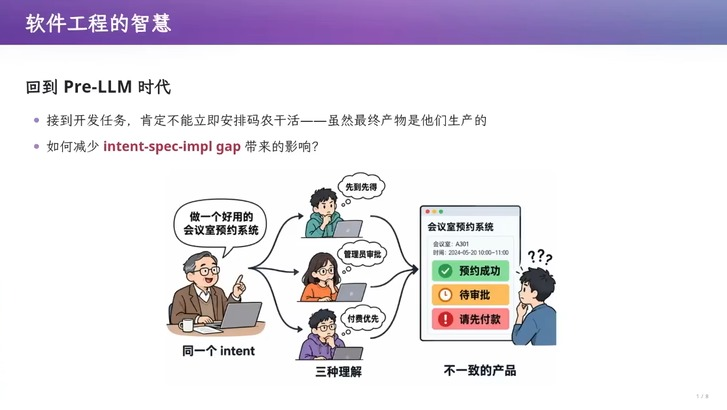
\includegraphics[width=\textwidth]{figures/fig_23_intent_three_interpretations.jpg}
\caption{软件工程的智慧：回到 Pre-LLM 时代。同一个 intent（“做一个好用的会议室预约系统”）被三个人理解成先到先得、管理员审批、付费优先，得到不一致的产品\vtag}
\end{figure}
\srcnote{00:50:45--00:51:00}

上图是课件对这个问题的概括：同一个 intent，三种理解，得到不一致的产品。那么，从一个空仓库出发时，应该怎样组织开发？1970 年软件工程刚刚诞生，还没有 MVP 的说法，也没有大语言模型。

\subsection{Royce 的问题：如何按时、不超预算地交付大型软件}

Winston Royce 的论文题为 \emph{Managing the Development of Large Software Systems}（1970），讲者称之为软件工程领域的开山之作。课件标注了它的背景：航天器任务规划、指令与飞行后分析，时间和存储都有硬约束。这篇论文画出了后来被称为“瀑布模型”的经典阶段图；而原文在这张图之后就指出，这样的实施方式风险很高，容易失败。

\begin{figure}[H]
\centering
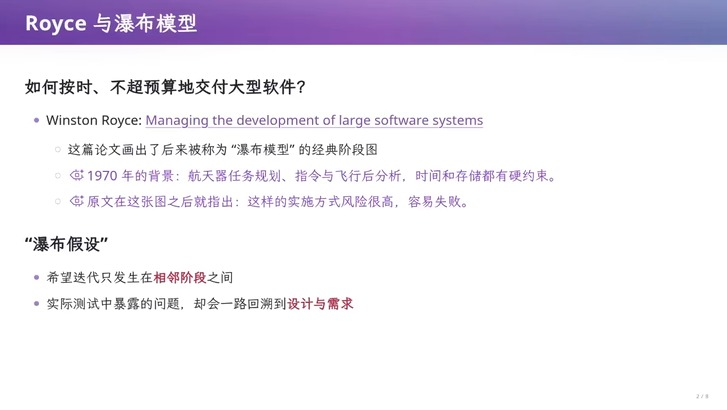
\includegraphics[width=\textwidth]{figures/fig_24_royce_waterfall_slide.jpg}
\caption{Royce 与瀑布模型：如何按时、不超预算地交付大型软件？“瀑布假设”——希望迭代只发生在相邻阶段之间，实际测试中暴露的问题却会一路回溯到设计与需求\vtag}
\end{figure}
\srcnote{00:51:30--00:51:45}

课件把 Royce 批评的对象称为“瀑布假设”：希望迭代只发生在相邻阶段之间；可实际测试中暴露的问题，却会一路回溯到设计与需求。讲者在课上打开百度搜索“瀑布模型”，说明几乎每一门软件工程课都会展示一张从上到下、逐级流下的阶段图——而这张图正出自 Royce 的论文。

\subsection{细读原文：两步就够的小程序与七步的大系统}

讲者没有读教科书的转述，而是让自己的“AI 读论文助手”把论文入库，得到按页切分、图片内嵌的 Markdown 版本 \texttt{royce.md}，再在命令行里逐页阅读。论文的 Figure 1 只有两个框：ANALYSIS 和 CODING。Royce 说，一个小到交给使用者本人的内部程序，这两步就够了。讲者的类比是：这就是同学们写的 Online Judge 程序。

\begin{figure}[H]
\centering
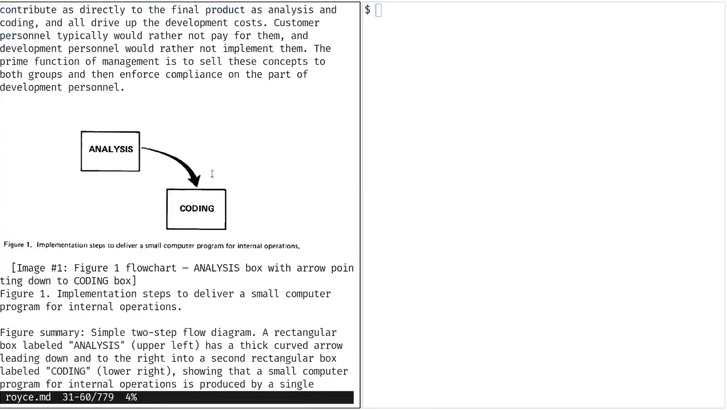
\includegraphics[width=\textwidth]{figures/fig_25_royce_fig1.jpg}
\caption{royce.md 中的 Royce 原文 Figure 1：交付小型内部程序只需 ANALYSIS → CODING 两步；原文随后说明，大型系统里客户和开发人员都不愿为其他步骤付费或执行\vtag}
\end{figure}
\srcnote{00:53:45--00:54:00}

原文 Figure 2 把流程扩展为七个阶段：SYSTEM REQUIREMENTS、SOFTWARE REQUIREMENTS、ANALYSIS、PROGRAM DESIGN、CODING、TESTING、OPERATIONS。讲者概括为：需求到系统需求、软件需求，分析，设计，编码，测试，上线运维。原文对它的第一个评价是：随着设计推进，每一步与前后相邻的步骤之间有迭代，而与更远步骤的迭代很少；这样每次改动的范围可以被控制住。

\begin{figure}[H]
\centering
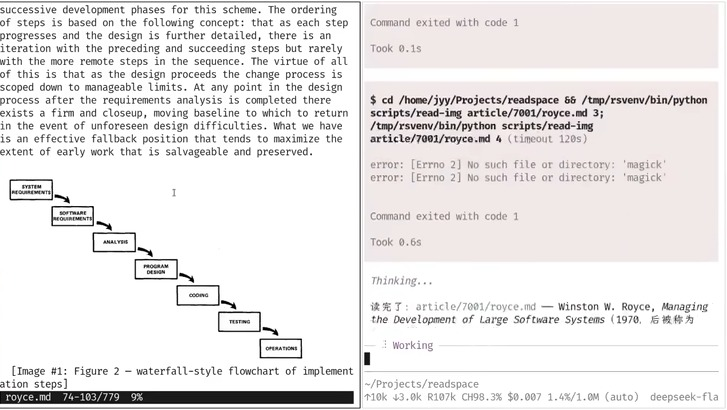
\includegraphics[width=\textwidth]{figures/fig_26_royce_fig2_waterfall.jpg}
\caption{royce.md 中的 Royce 原文 Figure 2：瀑布式的七阶段流程图，后来被称为“瀑布模型”\vtag}
\end{figure}
\srcnote{00:55:15--00:55:30}

\subsection{测试是第一个“物理事件”}

紧接着，Royce 说他相信这个概念，但按图实施“有风险，容易失败”。讲者转述了原文的理由，并把它称作全文最锋利的观察：测试是整个链条上第一个“物理事件”。设计阶段只有报告；在程序被真正写出来之前，它都不能运行。课件的写法是：Testing 是 timing、storage、I/O 第一次“被经历”、而非“被分析”的地方；这些系统行为难以在实际运行前精确分析，一旦实际运行不满足约束，局部修补代码往往不够。

\begin{figure}[H]
\centering
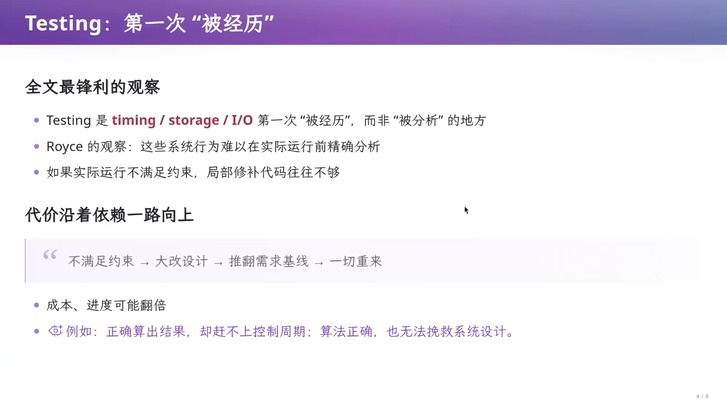
\includegraphics[width=\textwidth]{figures/fig_30_testing_first_experienced.jpg}
\caption{Testing：timing / storage / I/O 第一次“被经历”；代价沿着依赖一路向上——不满足约束 → 大改设计 → 推翻需求基线 → 一切重来\vtag}
\end{figure}
\srcnote{01:07:15--01:07:30}

讲者从人性角度补充了这一点：当东西还不能运行的时候，人都会“随便做做”。文档就是例子——同学们写实验文档时，对它的正确性有 guarantee 吗？最多是 best effort。文档写完就放在那里，代码和设计改了、文档不一致，也就放在那里，没有强约束。只有测试时程序真正跑起来，你才知道它的行为是什么。如果 intent 到 spec 到 impl 的过程中发生了漂移，到测试时才发现，就意味着要回到前面修改，而这正是超期和超支的源头。课件把代价的传播写成一条链：
\begin{center}
不满足约束 $\rightarrow$ 大改设计 $\rightarrow$ 推翻需求基线 $\rightarrow$ 一切重来
\end{center}
其结果是成本、进度可能翻倍。课件举的例子是：算法正确、结果正确，却赶不上控制周期，算法正确也无法挽救系统设计。

\subsection{Do It Twice：Royce 的补救方案}

既然风险最终都在测试时爆炸，讲者说，所有补救的本质都是把发现问题的时间点提前。Royce 的建议包括设计先行、文档做足，其中最经典的是 “do it twice”：先做一个 preliminary pilot program（初步的试验程序），它不完备，但能体现系统功能；它可能失败，但迭代成本很低，失败的教训可以反馈到正式系统的设计上。

\begin{figure}[H]
\centering
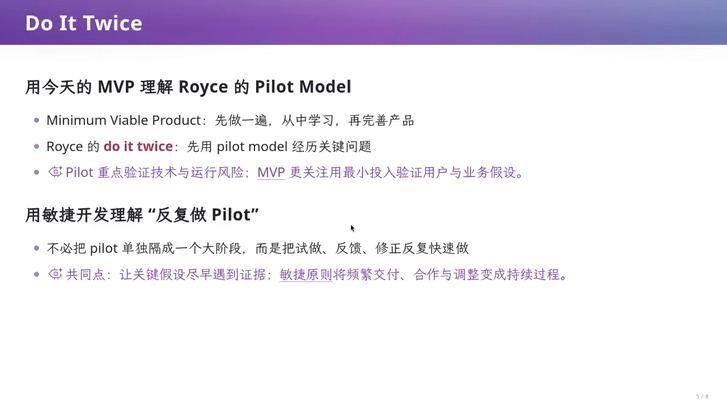
\includegraphics[width=\textwidth]{figures/fig_31_do_it_twice.jpg}
\caption{Do It Twice：用今天的 MVP 理解 Royce 的 Pilot Model；用敏捷开发理解“反复做 Pilot”\vtag}
\end{figure}
\srcnote{01:07:45--01:08:00}

讲者的评论是：“这是什么？这就是 minimum viable product。”课件同时标出了两者的区别：Pilot 重点验证技术与运行风险；MVP 更关注用最小投入验证用户与业务假设。用敏捷开发的眼光看，也不必把 pilot 单独隔成一个大阶段，而是把试做、反馈、修正反复快速做；两者的共同点是让关键假设尽早遇到证据，敏捷原则把频繁交付、合作与调整变成了持续过程。

论文最后给出了 Royce 推荐的完整开发过程（Figure 10）：中心是一个大的迭代环（初步设计 → 分析 → 程序设计 → 编码 → 测试 → 运行），周围是评审节点，客户在整个开发周期中持续参与，反馈箭头从每一个阶段回到更早的阶段。

\begin{figure}[H]
\centering
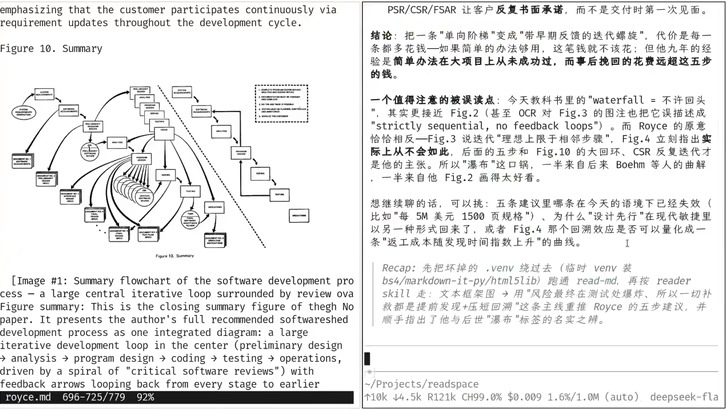
\includegraphics[width=\textwidth]{figures/fig_28_royce_fig10_summary.jpg}
\caption{royce.md 中的 Royce 原文 Figure 10（Summary）与 Agent 的结论：把单向阶梯变成带早期反馈的迭代螺旋\vtag}
\end{figure}
\srcnote{01:03:00--01:03:15}

\begin{warningbox}{被误读最严重的一篇论文}
讲者说，最有意思的是：大家学软件工程都学瀑布模型，而这篇文章实际上是批判瀑布模型的。Agent 的读后结论也指出，今天教科书里的 “waterfall = 不许回头” 其实只取了 Figure 2 的“严格顺序、没有反馈环”，而 Royce 的原意恰好相反：Figure 3 说迭代“理想上限于相邻步骤”，Figure 4 立刻指出实际上并不会如此；后面的五步建议和 Figure 10 的大回环，才是作者的主张。讲者的教训是：一个东西经过多次消化以后，你得到的可能已经不是那个东西了。
\end{warningbox}

讲者也强调了这篇论文的时代条件：1970 年“什么也没有”，只能从 first principle 思考。而论文描述的流程今天依然成立：你总是从空项目开始，不管用什么版本控制工具，都要先想清楚要干什么，再大概想想架构，再写代码；不管写代码的是软件工程师还是 AI，这个流程都成立。

\subsection{本章小结}

Royce 论文的真正论点是：瀑布式的单向流程之所以危险，是因为程序第一次真正运行（测试）发生得太晚，而那时发现的问题会沿着依赖一路回溯到设计和需求。他的补救是先做一遍 pilot，让关键假设提前碰到证据——这正是今天 MVP 与敏捷开发的思想。下一节看讲者是怎样读这篇论文的，以及这种读法本身对学习意味着什么。

\section{AI 时代的一手信息：谁来决定知识怎样压缩}

这一节回答一个由读 Royce 论文引出的学习问题：既然教科书把瀑布模型讲歪了，今天的学习者应该怎样获取知识？讲者的主张是：AI 让每个人都能直接读一手材料，并按自己的需要压缩知识。

\subsection{讲者的 AI 阅读助手}

讲者读论文的方式是：找到论文链接，对 Agent 说“入库这个 paper”，得到一个按页切割、所有图片以 Markdown 形式嵌入的文字整理版；再用自己写的命令行工具打印文本、提取图片，用一个类似 \texttt{less} 的阅读器在终端里逐页读，遇到问题直接问 Agent。课上他让 DeepSeek Flash 模型在后台读 Royce 论文，并让它解释“瀑布模型在软件工程里到底是怎样被误读的”。Agent 甚至能追溯误读链：教材一级一级转述，最后到学生手里的软件工程教材上，是怎样一步步曲解的。讲者评价这个解释“还挺 make sense 的”，同时提醒：你也可以选择不相信 AI，继续追问，或者换一个联网更好的模型。

\begin{figure}[H]
\centering
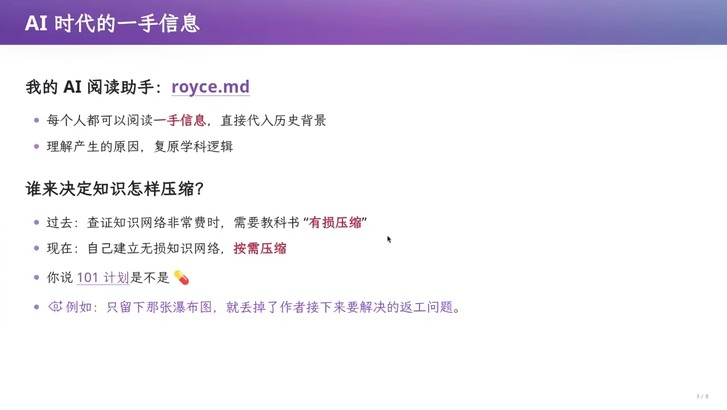
\includegraphics[width=\textwidth]{figures/fig_27_ai_firsthand_info.jpg}
\caption{AI 时代的一手信息：我的 AI 阅读助手 royce.md；谁来决定知识怎样压缩？过去需要教科书“有损压缩”，现在可以自己建立无损知识网络、按需压缩\vtag}
\end{figure}
\srcnote{01:01:00--01:01:15}

Agent 的回答里有一句讲者很认同的话：瀑布“好画、好背、好出题”，是“史上最好用的反派”，每一个新方法都拿它作对照。讲者补充说，它本身就是错的：1970 年的原文已经告诉你不能瀑布，要先做 MVP。

\subsection{从“有损压缩”到“按需压缩”}

讲者用“知识压缩”解释这种变化。过去查证一个知识网络几乎不可能：要去图书馆翻很多资料，索引机制也不好，找到精确的资料要花无穷多时间。所以那时的人不可能通过一手资料学习，必须经过教科书做知识的有损压缩。好的教科书作者读过一手信息，又能共情学生，知道学生哪里会不明白，压缩时对读者的损失很小；差的教科书则被戏称为“防自学”的教科书。

今天情况变了。讲者说，作为老师，他不需要再做压缩，因为任何压缩对每个人都是有损的，而且对不同的人损失的是不同部分；一对一教学才能做最适合你的压缩。现在只需要把知识的脉络拆解成一个个“发现的点”，把每个点和它的原文交给学习者，由学习者借助 AI 做属于自己的压缩。课件举的例子正是瀑布模型：只留下那张瀑布图，就丢掉了作者接下来要解决的返工问题。

\begin{knowledgebox}{讲者对课程建设的判断}
课件上有一句“你说 101 计划是不是”（后面是一个药丸表情）。讲者说，在查证知识网络非常费时的年代，如果真正的专家能帮你做好压缩，这种投入毫无疑问有价值；但在 AI 时代，一个领域里投入的百万、千万甚至上亿元，可能被一个模型——“可能是 DeepSeek Flash 这样的模型”——碾过去。这是讲者的个人判断。
\end{knowledgebox}

\subsection{读经典的方法：带着今天的经验回到当年的问题}

讲者给出的读经典理由是：经典记录了一个领域最初遇到的、也最根本的问题，以及它怎样找到出路；即便今天已经过时，信息量通常仍然巨大，而且在今天的背景下反而非常容易理解。他说自己读 Royce 原文时，两页纸的教材读两遍没懂的东西，一回到原文马上就懂了。

\begin{figure}[H]
\centering
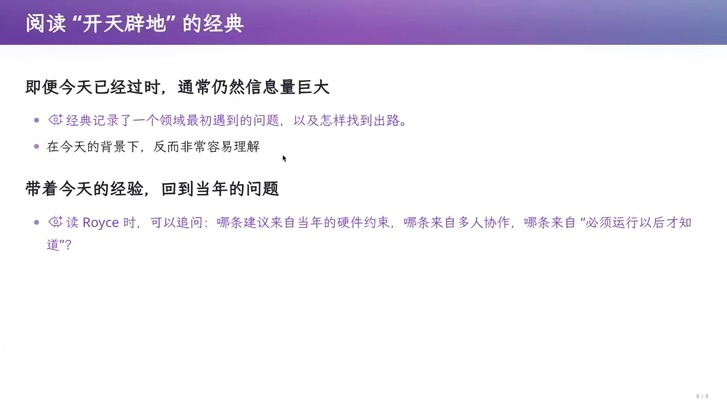
\includegraphics[width=\textwidth]{figures/fig_34_read_classics.jpg}
\caption{阅读“开天辟地”的经典：即便今天已经过时，信息量仍然巨大；读 Royce 时可以追问哪条建议来自当年的硬件约束、哪条来自多人协作、哪条来自“必须运行以后才知道”\vtag}
\end{figure}
\srcnote{01:14:45--01:15:00}

课件建议的读法是带着今天的经验回到当年的问题。读 Royce 时可以追问：哪条建议来自当年的硬件约束，哪条来自多人协作，哪条来自“必须运行以后才知道”？讲者还指出，今天正确的 practice 可以映射到过去，过去正确的 first principle 也可以映射到今天。他喜欢这些早期工作的原因是：很多图灵奖级别的工作，是在大家完全不知道该怎么做的时候确立了一个 first principle；在它上面长出了后来的许多分支。当然也有有趣的反例：某个起点方向想错了，可能把全人类都带歪，就像直流电与交流电之争。

\subsection{本章小结}

AI 降低了查证一手材料的成本，使“谁来压缩知识”从教科书作者转移到学习者自己。读经典的价值在于看到一个领域最初的问题和出路，而 AI 让这种阅读变得可行。下一节讲者示范另一种读法：用自己熟悉的计算机科学概念重新解释 Royce 的模型。

\section{瀑布模型就是数据依赖图：MVP、TDD 与敏捷}

这一节回答：瀑布、Pilot、MVP、TDD、敏捷开发看起来是几种不同的方法，能否用一个统一的模型比较它们？讲者给出的是他作为计算机科学背景的人自己的理解：把开发过程看作一张数据依赖图（data dependency graph），修改上游节点有代价。他说“这是我自己的理解，我觉得还是自洽的”。

\subsection{把每个阶段看成一个程序}

讲者先做了一个类比：把人看成程序。从需求分析到系统设计、系统实现、测试验证、交付维护，每个阶段都可以想象成一个 program，它读入上游的产物（artifact），产生下游的产物。他解释这个类比为什么说得通：人脑也是神经网络，人也会做 chain of thought——他自己想问题时，即使不说话，也会用语言对齐脑内的思维链。

这样看，整个开发过程的产物构成一张有向无环图。需求里有好几个点，彼此可能有关联，也可能没有；设计中的某个部分依赖其中几个需求点，实现又依赖设计，关联关系一路传递下去。

\begin{figure}[H]
\centering
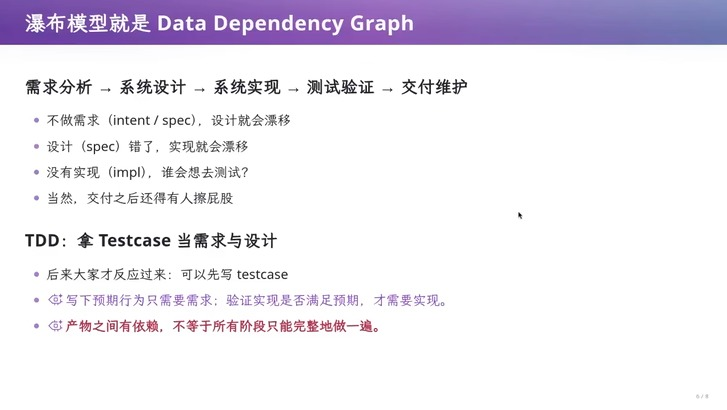
\includegraphics[width=\textwidth]{figures/fig_32_data_dependency_graph.jpg}
\caption{瀑布模型就是 Data Dependency Graph：需求分析 → 系统设计 → 系统实现 → 测试验证 → 交付维护；TDD 拿 Testcase 当需求与设计\vtag}
\end{figure}
\srcnote{01:13:15--01:13:30}

课件把每个阶段缺失时的后果写成四句话：不做需求（intent / spec），设计就会漂移；设计（spec）错了，实现就会漂移；没有实现（impl），谁会想去测试？当然，交付之后还得有人“擦屁股”。

\begin{importantbox}{返工代价为什么高}
在依赖图里，一旦测试发现错误，往上追溯发现是某几个设计错了，那么所有依赖这些设计的产物都要作废重做。这就解释了 Royce 说的“缺陷被发现得越晚，返工代价越大”。讲者用 OJ 的经历说明：头脑一热想了一个算法，没验证就去写代码，写完发现样例不对，再对着样例一跑，才发现整个算法都错了——这就是一次典型的瀑布模型失败。
\end{importantbox}

\subsection{缩短反馈路径：从广度优先到深度优先}

如果修改上游节点代价很高，讲者说很自然的对策是“把它割小”：不要一次性产生大量依赖。瀑布模型相当于用广度优先（BFS）的方式构建软件——先做完第一层，再做第二层；MVP 和敏捷开发则变成深度优先（DFS）——先把优先级最高的那条依赖链走通，走通以后再不断向旁边扩展，一轮一轮迭代。讲者说：“这不就是敏捷开发吗？”

\begin{figure}[H]
\centering
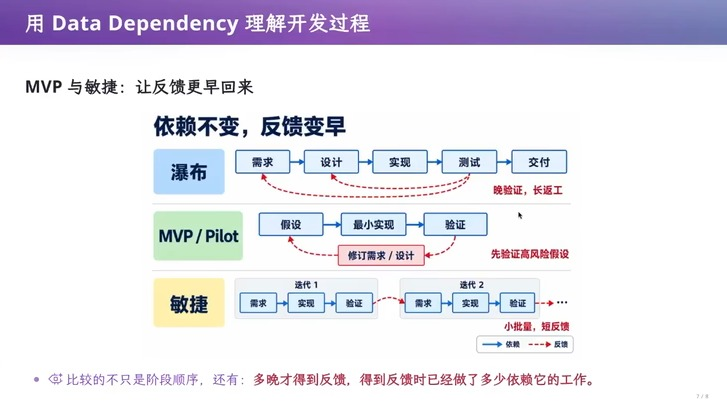
\includegraphics[width=\textwidth]{figures/fig_33_dd_feedback_diagram.jpg}
\caption{用 Data Dependency 理解开发过程：依赖不变，反馈变早。瀑布晚验证、长返工；MVP/Pilot 先验证高风险假设；敏捷小批量、短反馈\vtag}
\end{figure}
\srcnote{01:14:00--01:14:15}

上图把三种流程画在同一套依赖关系上，下表 是对这张图的文字整理。课件的结论是：比较的不只是阶段顺序，还有“多晚才得到反馈”，以及“得到反馈时已经做了多少依赖它的工作”。

\begin{table}[H]
\centering
\small
\begin{tabular}{p{0.14\textwidth}p{0.36\textwidth}p{0.38\textwidth}}
\toprule
流程 & 依赖链 & 反馈特点 \\
\midrule
瀑布 & 需求 → 设计 → 实现 → 测试 → 交付 & 晚验证，长返工：测试发现的问题要一路退回设计甚至需求 \\
MVP / Pilot & 假设 → 最小实现 → 验证，反馈回到“修订需求 / 设计” & 先验证高风险假设 \\
敏捷 & 迭代 1（需求 → 实现 → 验证）→ 迭代 2 → …… & 小批量，短反馈 \\
\bottomrule
\end{tabular}
\caption{三种开发流程在同一依赖关系上的反馈差异（据 01:14:00 课件图整理）}
\label{tab:flows}
\end{table}

讲者进一步把这个模型和 intent--spec--impl 对应起来：瀑布模型的前期阶段，比如需求阶段，对应把 intent 确定下来；设计阶段基本确定 spec（需求阶段也会做一点）；编码和测试阶段才是 implementation。因为每一层之间有 gap，每一个 intent 都会拆成好多个小点，并对后面的产物产生依赖，所以做 MVP、做敏捷、做 TDD“显然是一个正确的事情”。他的总结是：“这就是软件工程，没有什么真正困难的”——越早得到反馈，就越能消除路线上的不确定性。

\subsection{TDD：拿测试用例当需求与设计}

TDD（Test Driven Development，测试驱动开发）是讲者用来展示“今天的 practice 可以映射回过去”的例子。课件的说法是：后来大家才反应过来，可以先写 testcase；写下预期行为只需要需求，验证实现是否满足预期才需要实现。讲者说，在 TDD 的意义上，“设计先行”就是先把测试用例定好：输入这个，就应该经历这个流程、输出这个。课件还特意强调：产物之间有依赖，不等于所有阶段只能完整地做一遍。

讲者让 Agent 把 Royce 的建议逐条映射到 TDD，得到了下表（据画面整理了可见的三行）。Agent 的总体判断是：Royce 的五条建议全是“这条判断”的实例，TDD 不是新原理，而是把这条判断的回路长度从“月”压到了“秒”。

\begin{figure}[H]
\centering
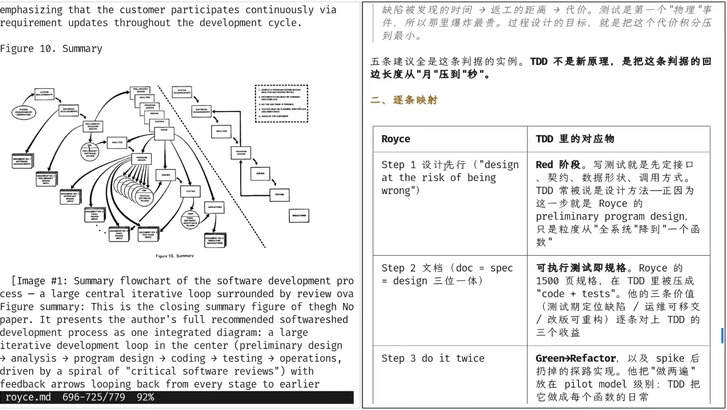
\includegraphics[width=\textwidth]{figures/fig_29_royce_tdd_mapping.jpg}
\caption{Agent 生成的映射表：Royce 的建议与 TDD 中的对应物\vtag}
\end{figure}
\srcnote{01:06:15--01:06:30}

\begin{table}[H]
\centering
\small
\begin{tabular}{p{0.30\textwidth}p{0.60\textwidth}}
\toprule
Royce 的建议 & TDD 里的对应物 \\
\midrule
Step 1 设计先行（“design at the risk of being wrong”） & Red 阶段：写测试就是先定接口、契约、数据形状、调用方式；TDD 常被说是设计方法，因为这一步就是 Royce 的 preliminary program design，只是粒度从“全系统”降到“一个函数” \\
Step 2 文档（doc = spec = design 三位一体） & 可执行测试即规格：Royce 的 1500 页规格，在 TDD 里被压成“code + tests”；他的三条文档价值（测试期定位缺陷、运维可移交、改版可重构）逐条对上 TDD 的三个收益 \\
Step 3 do it twice & Green → Refactor，以及 spike 后扔掉的探路实现：把“做两遍”放在 pilot model 级别，TDD 把它做成每个函数的日常 \\
\bottomrule
\end{tabular}
\caption{Royce 建议与 TDD 的对应关系（据 01:06:15 画面中 Agent 输出整理，只收录画面可见部分）}
\label{tab:royce-tdd}
\end{table}

\subsection{同一个 first principle，不同的解释}

讲者由此强调了个性化学习：每个人都可以用自己熟悉的概念理解同一个模型。他说自己是做操作系统的人，所以会很自然地用计算机科学里的概念解释这个世界；其他人也可以有自己的解释。他说，经典的价值在于在方向上找到了出路，即使后来可以援引其他概念（比如数据依赖）解释得更好；而“数据依赖”这个视角在整个软件工程发展史上都可以一路推下去，导出更多概念。

\subsection{本章小结}

把开发过程看成产物之间的数据依赖图，返工代价就是“上游修改使下游作废”的代价。瀑布、Pilot、MVP、TDD、敏捷的区别，不在于有没有需求、设计、实现这些阶段，而在于多早得到反馈、得到反馈前已经堆积了多少依赖。接下来的问题是：除了调整流程，软件工程还为每个阶段发明了哪些方法和工具来减少返工？

\section{方法与工具：为每个阶段建立可检查的“语言”}

这一节回答：在调整开发流程之外，软件工程为需求、设计、编码、测试、维护各个阶段发明了什么？讲者的总结是：为每个阶段创建方法学和工具，尽可能减少返工的概率；而这些方法的共同方向，是把原本只能用自然语言表达的东西，逐步变成有确定语义、可以检查的“语言”。

\subsection{为每个阶段创建方法学和工具}

\begin{figure}[H]
\centering
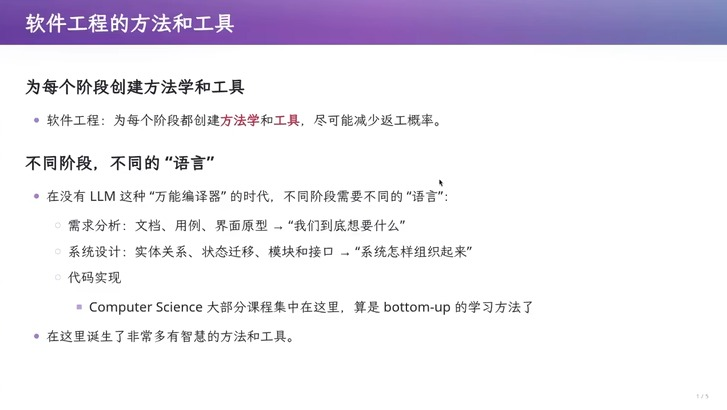
\includegraphics[width=\textwidth]{figures/fig_35_methods_tools.jpg}
\caption{软件工程的方法和工具：为每个阶段创建方法学和工具，尽可能减少返工概率；不同阶段，不同的“语言”\vtag}
\end{figure}
\srcnote{01:23:00--01:23:15}

讲者从软件工程课上最让学生反感的东西讲起：checklist。上软件工程课时，老师让你写文档，附带一份很长的 checklist：这个有没有做到，那个有没有沟通过。做惯 OJ 题的同学会觉得这是 nonsense。可 checklist 实际上减少了失败的概率。比如清单最后总有一条“你是否和客户最后沟通过”；当你真的和客户沟通过并打上勾，你就大幅降低了 intent 不符合客户要求的概率。讲者说，这是一种方法，也是一种工具，而且是“有人文关怀的工具”，它没有任何代码。

今天做软件工程研究，更多是在有了代码以后做文章：能不能自动测试（讲者调侃这方面有“无穷多灌水的 paper”），代码里有没有 bad smell（坏味道）。例如等号左右从不写空格的代码，会被认为是不好的代码——这条规定在 AI 时代之前一直成立。讲者观察到一个变化：GPT-6 学会省 token 以后，会写出极难理解、把很多语句塞进一行的代码，而那个代码是对的，“我不知道它是怎么弄对的”；也许我们永远不应该去读那样的代码。

他也提醒准备读研的同学：做软件工程研究，大概率会落在一个很小的点上，比如针对某种 Java 代码 bad smell 的更好检测；深挖的同时不要忘了看树林，看这些经典。深度训练让人有更长的思维链，广度训练让人对整个世界有更好的感觉。

\subsection{不同阶段，不同的“语言”}

课件指出，在没有 LLM 这种“万能编译器”的时代，不同阶段需要不同的“语言”：需求分析用文档、用例、界面原型，回答“我们到底想要什么”；系统设计用实体关系、状态迁移、模块和接口，回答“系统怎样组织起来”；最后才是代码实现。课件还注明：计算机科学的大部分课程集中在代码实现这一层，算是一种 bottom-up 的学习方法。

讲者说，在 checklist 阶段，尤其在大语言模型之前，几乎不可能用编程语言写 checklist——那时是一个 docx 文档，打印出来存档，和客户沟通的记录可能是手写的。编程阶段才有编程语言。这里马上就出现了一个 gap：在设计阶段，1970 年的人没有一种语言帮助做设计，用的都是自然语言，也就是设计文档。讲者回忆自己学软件工程时就是先写需求文档，再写设计文档，按瀑布模型走。

\begin{warningbox}{文档的最大缺点}
讲者说，文档最大的缺点是：写文档的是人。人会产生“幻觉”，会写错字；更重要的是，两个人讲同一件事时无法对齐——你说的是这个，室友理解成了那个，要花很多时间沟通。所以从 first principle 出发，要“为设计阶段创建方法和工具、减少返工”，就需要一种介于自然语言和编程语言之间的设计语言，也就是某种 domain specific language。
\end{warningbox}

讲者认为 checklist 本身就是一种中间语言：它虽然是自然语言，但有格式规范，要求一条一条写，每一条必须打勾或打叉；它有一定的语义，虽然由人来检查，人对“勾”和“叉”的对齐，比对一篇文档的对齐更 formal（形式化）一些。沿着开发阶段往下，语言的形式化程度——也就是语义的确定性——越来越高，这恰好对应从 intent 到 spec 到 impl 逐步消除 gap 的过程。讲者说，理解了这一点，就开始理解软件工程这个学科了。

\begin{knowledgebox}{学习顺序的变化}
过去计算机专业的学习是 bottom-up 的：先学编程，先学怎么做码农，因为不理解代码就无法理解整个过程。讲者认为 AI 来了以后可以变：第一门课就可以先学做产品（product）。后面的事情 AI 可以做，你不需要控制质量也能设计出好的产品，只要有好的想法。这是讲者对未来课程设计的设想。
\end{knowledgebox}

\subsection{方法和工具的智慧：把规则变得可检查}

\begin{figure}[H]
\centering
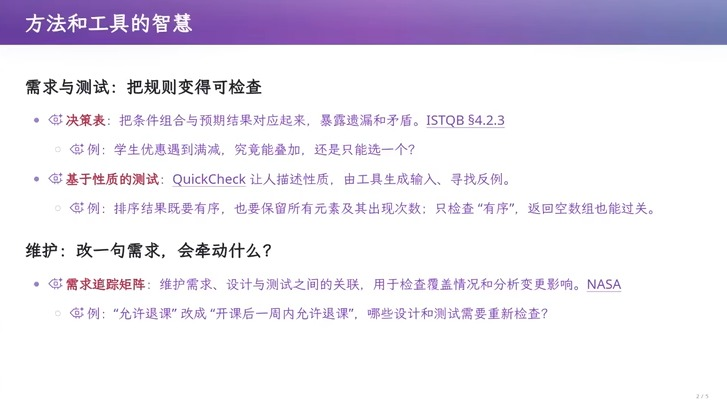
\includegraphics[width=\textwidth]{figures/fig_36_methods_wisdom.jpg}
\caption{方法和工具的智慧：需求与测试——决策表、基于性质的测试（QuickCheck）；维护——需求追踪矩阵\vtag}
\end{figure}
\srcnote{01:27:15--01:27:30}

课件列出了三种代表性方法，每种都对应一个具体例子（见下表）。

\begin{table}[H]
\centering
\small
\begin{tabular}{p{0.16\textwidth}p{0.36\textwidth}p{0.38\textwidth}}
\toprule
方法 & 做法 & 课件上的例子 \\
\midrule
决策表（ISTQB §4.2.3） & 把条件组合与预期结果对应起来，暴露遗漏和矛盾 & 学生优惠遇到满减，究竟能叠加，还是只能选一个？ \\
基于性质的测试（QuickCheck） & 让人描述性质，由工具生成输入、寻找反例 & 排序结果既要有序，也要保留所有元素及其出现次数；只检查“有序”，返回空数组也能过关 \\
需求追踪矩阵（NASA） & 维护需求、设计与测试之间的关联，用于检查覆盖情况和分析变更影响 & “允许退课”改成“开课后一周内允许退课”，哪些设计和测试需要重新检查？ \\
\bottomrule
\end{tabular}
\caption{需求、测试与维护阶段的三种方法（据 01:27:15 课件整理）}
\label{tab:methods}
\end{table}

讲者对决策表这类方法的评价有两面。作为“理科生”，他当年觉得这些“只有所有勾都打上才能进入下一阶段”的规定是 nonsense；有的 checklist 还要求把所有文档两两摆在一起审查一遍。但正是这种形式赋予了语义，避免了遗漏和矛盾，也避免了 gap 的漂移。“这都是智慧”；它们也失败过，而在管理团队的过程中形成的管理学经验，软件工程师同样可以学。

对 QuickCheck，讲者称它“基本上算是整个测试领域的开山鼻祖之一”，并解释了它背后的逻辑：从上到下的每一次翻译都会出错，从 specification 翻译到代码也一样；而且代码里还有许多隐含的 specification，比如程序不能 crash、不能有空指针、资源不能泄漏。如果能在代码里写一个 property，让它自动变成大量测试用例，全部通过时你对代码就更有信心。讲者说，你永远不知道一份代码对不对；测试做得越多、独立的质量保障越多，信心越大；只有写出形式化证明，信心才可能更大。

\subsection{需求追踪：把依赖图变成显式的链接}

需求追踪（traceability，可追溯性）是讲者在前几讲就提过的概念。他把它和数据依赖图联系起来：如果从文件系统或项目的角度看，一个软件就是一堆文件——\texttt{docs/} 下的一些 \texttt{.md}，\texttt{src/} 下的一些 \texttt{.ts}，还有一个 \texttt{README}。讲者说，按文件组织项目是因为文件系统先被大家用上而不得不做的一个 workaround；文件承载了整个软件，但文件本身并不记录需求、设计、代码之间的依赖。traceability 要求用链接或其他方式，让每一段代码和每一个需求点都对得上，需求与需求、需求与设计之间也对得上。所有这些都能对上、能互相交叉检验时，你对软件的质量就更有信心。

\begin{figure}[H]
\centering
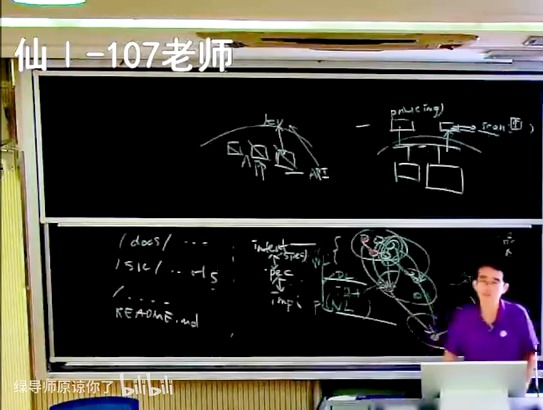
\includegraphics[width=0.62\textwidth]{figures/fig_37_board_traceability.jpg}
\caption{板书（摄像头区）：左侧是 \texttt{/docs/}、\texttt{/src/ ... .ts}、\texttt{README.md} 的文件视角，右侧是 intent → spec → impl 各层与它们之间的依赖图；上方是本讲前半段讲设备抽象时画的 printing / scan 与 API 草图\vtag}
\end{figure}
\srcnote{01:32:15--01:32:30}

讲者由此谈到“人的能力是有限的”这一前提。大学时每个人都想把自己变成世界上最厉害的码农，以为这样就能在软件企业找到好工作——这是社会给你的 contract。但从资本家的角度、或从完成一项任务的角度看，更重要的是：没有一个码农能单独完成项目，只能考虑要花多少钱、雇多少码农才能交付。讲者说，今天每个人都在当产品经理：你马上就可以有 2500 并发的 DeepSeek（他认为 DeepSeek“绝对算是一个相当资深的码农”），可你刚高考完，接受的训练里从来没有“怎么管 2500 个人”，这个 mindset 要改一改。

\subsection{本章小结}

软件工程为每个阶段发明的方法，本质上都是在自然语言和代码之间插入语义更确定的表达：checklist 让“有没有做到”可以打勾，决策表让条件组合无遗漏，基于性质的测试让隐含规格变成可执行检查，需求追踪让依赖关系变成显式链接。这些方法都假设人的能力有限、协作者之间难以对齐。下一节看这个方向走得最远的两次尝试：把契约写进编程语言，以及用 UML 统一建模语言。

\section{契约与 UML：用语言对齐意图}

这一节回答：能否设计一种语言，让意图在写代码之前就有确定的语义，从而在人和人之间、人和机器之间对齐？讲者讲了两条路线：把契约直接写进编程语言（Design by Contract），以及用一种统一的建模语言描述整个面向对象世界（UML）。他对后者的评价是“UML 已经死了”，但它的 first principles 一直在指导我们。

\subsection{契约编程：调用者与实现者各自负责什么}

Design by Contract（契约式编程，也译作面向契约的编程）来自 Bertrand Meyer 设计的 Eiffel 语言。课件的解释是：像人类合作中的契约一样，接口写清双方的义务与权利。其中前置条件由调用者保证，是调用前必须满足的使用条件；后置条件由实现者保证，是前置条件成立时正常返回后的结果。讲者说，Eiffel 在 1986 年左右就提出要把 Hoare 三元组直接写进代码。Hoare 三元组是程序验证中描述“前置条件—程序—后置条件”关系的标准记号：

\begin{equation}
\{P\}\ C\ \{Q\}
\end{equation}
\begin{itemize}
  \item $P$：前置条件（precondition），执行前假定成立的断言；
  \item $C$：一段程序（比如一个函数体）；
  \item $Q$：后置条件（postcondition），若 $P$ 成立且 $C$ 正常结束，执行后必定成立的断言。
\end{itemize}

\begin{figure}[H]
\centering
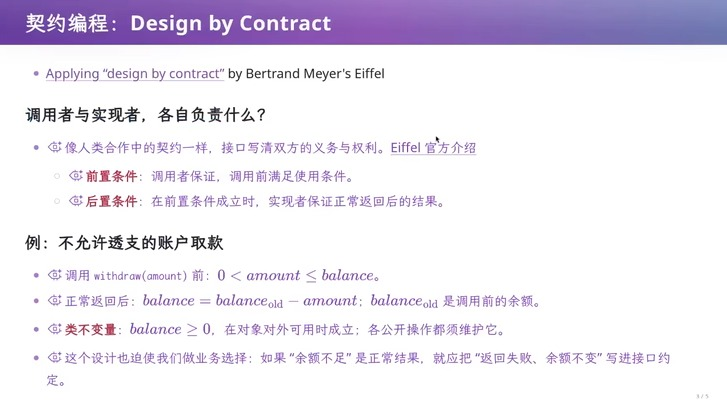
\includegraphics[width=\textwidth]{figures/fig_38_design_by_contract.jpg}
\caption{契约编程 Design by Contract：调用者与实现者各自负责什么；例子是不允许透支的账户取款\vtag}
\end{figure}
\srcnote{01:28:15--01:28:30}

课件用一个不允许透支的账户取款 \texttt{withdraw(amount)} 说明三类契约。调用前的前置条件是
\begin{equation}
0 < \mathit{amount} \le \mathit{balance}
\end{equation}
\begin{itemize}
  \item $\mathit{amount}$：本次取款金额，由调用者传入；
  \item $\mathit{balance}$：调用时账户的余额。
\end{itemize}
正常返回后的后置条件是
\begin{equation}
\mathit{balance} = \mathit{balance}_{\mathrm{old}} - \mathit{amount}
\end{equation}
\begin{itemize}
  \item $\mathit{balance}$：返回后的余额；
  \item $\mathit{balance}_{\mathrm{old}}$：调用前的余额；
  \item $\mathit{amount}$：本次取款金额。
\end{itemize}
此外还有类不变量（class invariant），在对象对外可用时成立，各公开操作都必须维护它：
\begin{equation}
\mathit{balance} \ge 0
\end{equation}
\begin{itemize}
  \item $\mathit{balance}$：任何一次公开操作前后的账户余额。
\end{itemize}

课件点出了这个设计的另一个作用：它迫使我们做业务选择。如果“余额不足”是正常结果，就应该把“返回失败、余额不变”写进接口约定。讲者补充说，写第一个 MVP 时你一定不会管这些事，要么让它 crash，要么假设它永远不会发生，把它排除在 specification space 之外；但当软件不断向后演进，contract 就变得非常重要。

\subsection{把契约写进语言：Eiffel 与今天的验证工具}

Eiffel 的“上古语法”把接口文档、前置条件、实现和后置条件写在同一个函数定义里：

\begin{lstlisting}[caption={Eiffel 的契约语法骨架（摘自下图课件）}]
function(args) is
    -- Comment
require
    Precondition
do
    Routine
ensure
    Postcondition
end
\end{lstlisting}

讲者逐段解释：\texttt{function ... is} 之后先写文档，说明这个函数是干什么的；\texttt{require} 是前置条件；\texttt{do} 是代码实现；\texttt{ensure} 是做完以后能够保证什么。Eiffel 鼓励你先不写 \texttt{do} 部分，而是先把各个模块的文档、precondition、postcondition 写出来；写这些的时候，你会自然地关联到设计，比如余额不足到底该怎样处理。课件补充：契约既是接口文档，也能在开启断言检查时检验本次执行。

\begin{figure}[H]
\centering
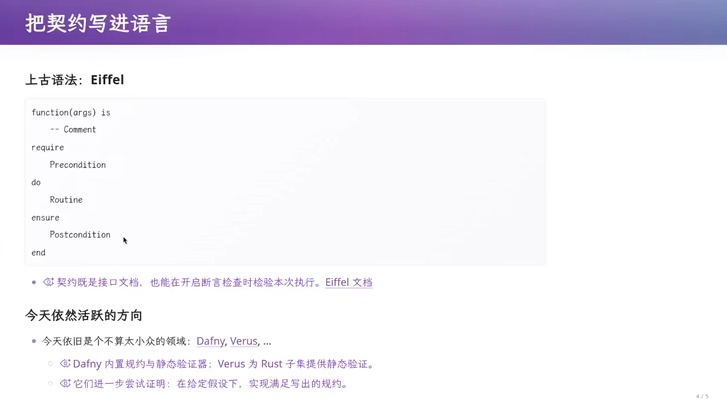
\includegraphics[width=\textwidth]{figures/fig_39_eiffel_contract.jpg}
\caption{把契约写进语言：上古语法 Eiffel；今天依然活跃的方向——Dafny、Verus 等\vtag}
\end{figure}
\srcnote{01:32:15--01:32:30}

讲者说，这么多年软件工程研究者做的事，就是在 spec 这一层“横跳”：从自然语言，到半自然的语言，到可以写逻辑公式、不需要代码就能检验逻辑（比如函数调用链上逻辑能否成立）的语言，再到今天的编程语言。这依然是非常活跃的方向。课件列出了今天仍不算小众的领域：Dafny 内置规约与静态验证器，Verus 为 Rust 子集提供静态验证，它们进一步尝试证明：在给定假设下，实现满足写出的规约。

\begin{importantbox}{讲者的一个预言}
讲者说，ChatGPT 出来之前他在操作系统课上就预言过：大约 30 年后，如果程序里有一个 assert——可以是前置条件、后置条件，也可以是和业务逻辑相关的断言，比如双向链表往前走再往后走总能回到自己——只要编译器不能证明它成立，程序就不能通过编译；能通过编译就百分之百保证它成立。到那时，连 property-based test 都不需要了，直接把 property 写进去让工具证明即可。以现在的进展看，他认为可能不需要 30 年，从那个时间点算 10 年或 15 年就能解决。这是讲者的预测。
\end{importantbox}

讲者的理由是：AI 来了以后，软件工程会发生很大变化。自然语言“对不齐”的问题、checklist 不好检查的问题都解决了，只剩下“我没有想清楚、没有说清楚”的 gap；一旦想清楚、说清楚，也许真的都能解决。

\subsection{UML：统一整个面向对象世界的中间语言}

在这条路线上的集大成者是 UML（Unified Modeling Language，统一建模语言）。它的想法很简单：世界这么复杂，不同层次用不同语言——实现时用 C 或 Java，设计时用专门的设计语言，需求阶段用各种 DSL——那能不能有一种中间语言，统一整个面向对象的世界？课件注明，UML 汇合了 Booch、OMT、OOSE 等方法，统一记号与语义，让团队和工具能使用共同的建模语言。

\begin{figure}[H]
\centering
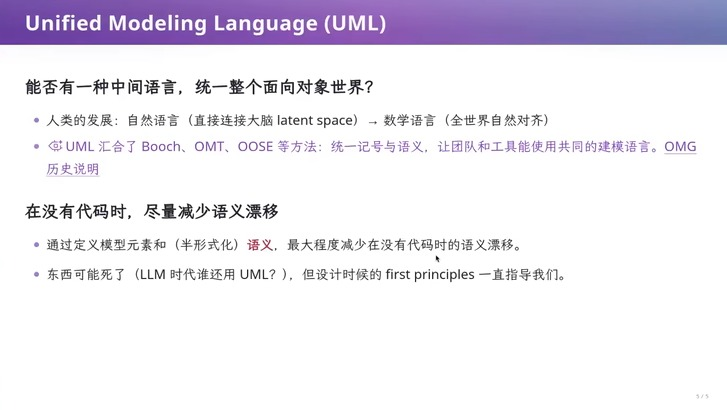
\includegraphics[width=\textwidth]{figures/fig_40_uml.jpg}
\caption{Unified Modeling Language：能否有一种中间语言统一整个面向对象世界？在没有代码时，尽量减少语义漂移\vtag}
\end{figure}
\srcnote{01:35:30--01:35:45}

讲者说这是一个非常有野心的目标：语义对齐，而这恰恰是人类天生没有做好的事。人类靠自然语言交流，而自然语言直接连接大脑的 latent space（潜在空间）。他的例子是：“我今天看到一个美女”，每个听者都在自己的 latent space 里构造了一个美女，但彼此都不一样；让不同模型用 Blender 画出来也各不相同。所以人类发明了数学语言：自然数从公理一点点构造出来，公理小到全人类基本都能对齐；一旦对齐，用 Peano 公理就能把整个计算机世界构建起来，计算机世界里同样的东西，语言是绝对对齐的。

UML 想做的，是去对齐自然语言世界里说不清的东西，比如需求和设计。百分之百对齐不可能，但它希望把能对齐的部分和不能对齐的部分剥离出来：通过定义模型元素和它们的（半形式化）语义，最大程度减少在没有代码时的语义漂移。讲者举了两个例子。类图的语义是确定的：有一个 class 叫 Student，里面有一个 field 叫 name，它就是 \texttt{Student.name}，可以变成源代码里的一个东西。顺序图说“按某个时序从前到后执行”，先后顺序就是绝对对齐的；如果写自然语言，一旦发生并发，谁先谁后、能不能并发都有歧义，而 UML 消除了这个歧义。

\begin{warningbox}{UML 为什么“死了”}
讲者认为 UML 已经死了：它的全部假设是自然语言和形式语言不能对齐，所以需要一层层中间语言；今天自然语言突然可以和任何东西对齐了，AI 可以直接和你确认。所以 UML 成了历史里的东西。课件的说法更谨慎：“东西可能死了（LLM 时代谁还用 UML？），但设计时候的 first principles 一直指导我们。”
\end{warningbox}

\subsection{让 AI 读 796 页的 UML 规范}

讲者说，上大学时学过 UML，“感觉没学懂”（他怀疑老师可能也不太懂），只有一些模糊印象，读 PhD 时读过一些 papers。这次他让 AI 帮他重读了整份 UML 规范。他的工具可以处理几千页的长文档，体验接近读 PDF。做法是：把规范 Dump 成文本，切成带 overlap 的片段，分给多个 SubAgent，每个 Agent 读 50 页，让它们提取其中的软件工程智慧，去掉不符合 AI 时代的不必要内容；他还把自己的全部 lecture notes 交给 AI，最后总结成课件。

\begin{figure}[H]
\centering
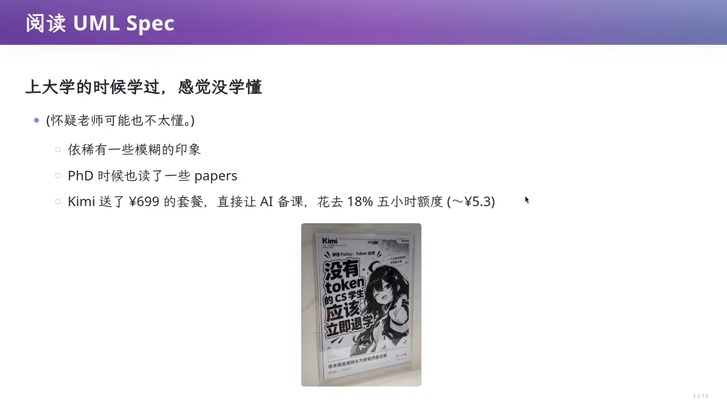
\includegraphics[width=\textwidth]{figures/fig_41_read_uml_spec.jpg}
\caption{阅读 UML Spec：Kimi 送了 ¥699 的套餐，直接让 AI 备课，花去 18\% 五小时额度（约 ¥5.3）\vtag}
\end{figure}
\srcnote{01:38:30--01:38:45}

成本方面，讲者说这可能算一个广告：Kimi 看到他的视频，送了他一个 699 元一个月的套餐。整个阅读花掉了 18\% 的 5 小时额度，折算下来约 5.3 元。
（讲者口头说规范有 700 页左右，课件上写的是 796 页。）

讲者由此提出一个“非常现实的问题”：拥有好模型和没有好模型的学生，学习效率和学习成本会有很大差距。他说如果用 GPT-6，价格可能差不多，因为它非常省 token，但质量可能好得多；对学习来说，一个 100 刀的 Codex 套餐大概够用。真正烧 token 的是维护大项目，上下文里会载入很多东西，100 万的上下文马上就填满；学习流程则可以用消化过的版本（digested version），不必像他这样把整个 UML spec 放进来。但如果要让所有人教育平权，没有那么多算力和资源怎么办？讲者的回答是“We don't know”，这可能是一个社会性问题。

\subsection{哪些意图必须显式钉死，哪些可以留白}

AI 对整份规范的总结被讲者概括为一句话：796 页规范从头到尾只在反复回答一个问题——哪些意图必须显式钉死，哪些可以留白；它的全部设计都是对这个问题的回答。UML 构造了一种半形式的语言，告诉你哪些东西可以在语义上确定下来，哪些可以不用。

\begin{figure}[H]
\centering
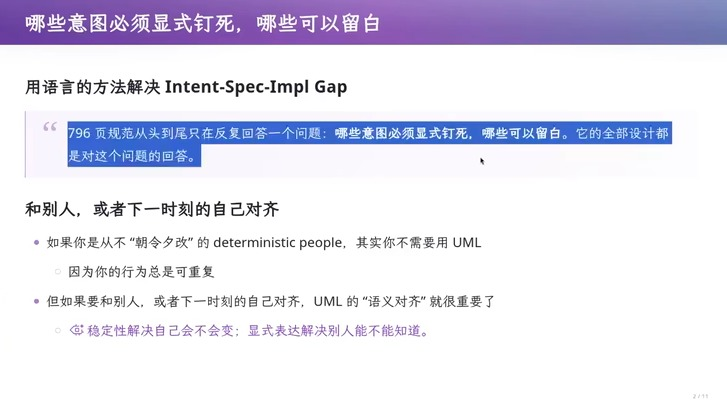
\includegraphics[width=\textwidth]{figures/fig_42_which_intents_pinned.jpg}
\caption{哪些意图必须显式钉死，哪些可以留白：用语言的方法解决 Intent-Spec-Impl Gap；和别人，或者下一时刻的自己对齐\vtag}
\end{figure}
\srcnote{01:39:15--01:39:30}

它解决的是对齐问题：人和人之间，甚至你和下一时刻的自己之间。课件写道：如果你是从不“朝令夕改”的 deterministic people，其实不需要 UML，因为你的行为总是可重复；但如果要和别人、或者下一时刻的自己对齐，UML 的“语义对齐”就很重要了。稳定性解决“自己会不会变”，显式表达解决“别人能不能知道”。讲者的说法是：你不是 deterministic 的，今天想的和明天想的就不一样，所以你和你自己也对不齐。

\begin{figure}[H]
\centering
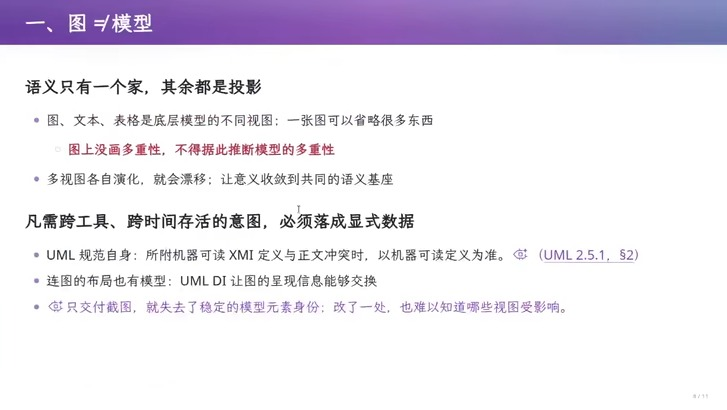
\includegraphics[width=\textwidth]{figures/fig_43_diagram_not_model.jpg}
\caption{一、图$\neq$模型：语义只有一个家，其余都是投影；凡需跨工具、跨时间存活的意图，必须落成显式数据\vtag}
\end{figure}
\srcnote{01:39:45--01:40:00}

讲者在下课前只展示了课件总结的第一条“图$\neq$模型”，其余留给同学自己看。这一条的内容是：语义只有一个家，其余都是投影。图、文本、表格是底层模型的不同视图，一张图可以省略很多东西，所以图上没画多重性，不能据此推断模型的多重性；多个视图各自演化就会漂移，要让意义收敛到共同的语义基座。凡需跨工具、跨时间存活的意图，必须落成显式数据：UML 规范自身规定，所附机器可读的 XMI 定义与正文冲突时，以机器可读定义为准（UML 2.5.1，§2）；连图的布局也有模型（UML DI），让图的呈现信息能够交换。课件的警示是：只交付截图，就失去了稳定的模型元素身份；改了一处，也难以知道哪些视图受影响。

\subsection{本章小结}

契约式编程和 UML 代表了同一个方向：在代码之前，用语义确定的语言把意图写下来，让人与人、人与机器、现在与将来的自己能够对齐。讲者认为 UML 作为工具已经过时，因为大模型让自然语言可以直接与形式语言对齐；但“哪些意图必须显式钉死、哪些可以留白”“语义只能有一个家”这些原则，在与 Agent 协作时仍然适用——Agent 同样需要知道哪些约束是硬的。

\section{总结与延伸}

\subsection{讲者的结论}

讲者在这一讲里反复回到同一个判断：软件难做，是因为 intent、spec、impl 之间有 gap；软件工程的全部历史，都可以看作人们为弥合这个 gap 发明的流程、方法和语言。1960 年代，客户不懂计算机能做什么，程序员不懂业务，需求又是人为设定、充满例外的；机器越强，承担的现实意图越多，gap 越大，于是有了软件危机和 1968 年的软件工程。Royce 1970 年的论文指出，程序第一次真正运行（测试）来得太晚，问题会一路回溯到需求，因此要“做两遍”；后来的 MVP、TDD、敏捷开发都在做同一件事：让关键假设尽早碰到证据。决策表、QuickCheck、需求追踪矩阵、契约式编程和 UML，则是在不同阶段用语义更确定的语言表达意图。

讲者对 AI 时代的判断是两面的。一方面，大模型让自然语言可以和任何形式语言对齐，checklist 可以自动检查，UML 这类中间语言“已经死了”，软件公司可能彻底消亡；另一方面，这些方法背后的 first principle 并没有消失，人仍然需要理解 AI 做了什么、判断它做得对不对，而能驾驭、能理解 AI 的人才能在“斩杀线”上升时留下来。他还提出了一个没有答案的问题：好模型会拉开学习效率和成本的差距，教育平权需要的算力从哪里来？

\subsection{本讲义的整理：一张统一的图}

本讲义把全讲内容压缩成下面几条，供复习时对照（这是笔记作者的整理，不是讲者原话）：

\begin{enumerate}
  \item \textbf{问题}：软件 = intent + spec + impl，三者之间的 gap 来自需求的人为性与定制化，且随机器能力增长而扩大。
  \item \textbf{代价模型}：开发产物构成一张数据依赖图，返工代价 = 被推翻的上游节点所拖累的全部下游工作。测试是第一个“物理事件”，所以瀑布式流程发现问题最晚、代价最高。
  \item \textbf{流程上的对策}：缩短反馈路径。Royce 的 pilot、MVP、TDD、敏捷只是反馈回路长短不同（Agent 的说法是从“月”压到“秒”）。
  \item \textbf{表达上的对策}：提高每一层表达的语义确定性。checklist、决策表、性质、追踪链接、契约、UML 模型，依次把“说不清”的意图变成可检查的数据。
  \item \textbf{AI 改变了什么}：生成实现几乎免费，自然语言与形式语言之间的翻译变得便宜；没有改变的是“想清楚、说清楚”的 gap，以及“哪些意图必须显式钉死”的判断。
\end{enumerate}

下表 把本讲出现的主要方法按“解决哪个 gap、靠什么反馈”排列。

\begin{table}[H]
\centering
\small
\begin{tabular}{p{0.20\textwidth}p{0.18\textwidth}p{0.50\textwidth}}
\toprule
方法 & 主要作用的环节 & 让什么更早碰到证据 / 变得可检查 \\
\midrule
Royce 的 pilot（1970） & intent → impl & 在正式系统之前先运行一次，暴露 timing、storage、I/O 等风险 \\
MVP & intent & 用最小投入验证用户与业务假设 \\
TDD & spec → impl & 测试用例先于实现，成为可执行的规格 \\
敏捷开发 & 全流程 & 小批量迭代，把频繁交付和调整变成持续过程 \\
checklist / 决策表 & intent → spec & 逐条确认、条件组合无遗漏 \\
QuickCheck & spec → impl & 由性质自动生成输入、寻找反例 \\
需求追踪矩阵 & 全流程 & 需求、设计、测试之间的依赖变成显式链接 \\
契约式编程 & spec → impl & 前置/后置条件与不变量写进代码，可检查或可证明 \\
UML & intent → spec & 半形式化语义，决定哪些意图钉死、哪些留白 \\
\bottomrule
\end{tabular}
\caption{本讲主要方法的对照（笔记作者整理）}
\label{tab:summary}
\end{table}

\subsection{与 Agent 协作时可以直接用的做法}

以下几条是笔记作者根据本讲内容整理的实践建议，均能在讲者的演示或论述中找到对应：
\begin{itemize}
  \item 给 Agent 一个\textbf{可验收的结果}，并尽量让它能自己观察结果（讲者说接一个摄像头，调标签浓度就不需要人）。
  \item 先定接口再让 Agent 实现（Office Assistant 的 \texttt{scan}/\texttt{print} 抽象），这样迭代可以局部进行。
  \item 需要多个 Agent 并行时，先由人划分任务（一个 Agent 管打印机，一个管扫描仪），不要指望它们自组织。
  \item 把业务规则里的例外写成显式约定，例如“余额不足时返回失败、余额不变”，否则 MVP 阶段它们会被默认排除在 spec 之外。
  \item 读经典或长文档时，让 AI 按页整理、分段阅读，但保留追问和换模型核对的习惯。
\end{itemize}

\subsection{边界与开放问题}

本讲的历史材料（NATO 会议、Apollo、Royce 论文、Eiffel、UML 规范）有原始文献可查；讲者对前沿实验室训练方式、软件公司消亡、UML 已死、形式化验证时间表的判断属于个人推断或预测，课上没有给出量化证据。几个值得继续追问的问题：
\begin{itemize}
  \item 如果 AI 让自然语言与形式语言“对齐”，那么谁来判断 AI 的翻译忠实于 intent？这是否只是把 intent--spec gap 换了个位置？
  \item 讲者预言“不能证明的断言就不能编译”。在 Dafny、Verus 之外，还需要什么条件，AI 才能为业务级断言生成可检查的证明？
  \item 数据依赖图的视角能否解释版本管理（上一讲）和需求追踪之间的关系：Git 记录了文件的历史，却不记录 intent 与 impl 的链接。
\end{itemize}

讲者预告，下一个实验会要求把第一个实验的系统连到一个物理设备上。按本讲的思路，这个实验可以先从一个 MVP 和一个干净的设备接口开始。


\end{document}
